\documentclass[usletter, 12pt]{article}
 
\usepackage{VB}
\usepackage{cleveref}
\usepackage{amsthm}
\usepackage{mdframed}
\usepackage{caption}
\usepackage{bbm}
\usepackage{rotating}

\newtheorem{theorem}{Theorem}
\newtheorem{lemma}{Lemma}
\newtheorem{proposition}{Proposition}
\newtheorem{corollary}{Corollary}
\newtheorem{definition}{Definition}


%\doublespacing

\begin{document}

\lhead{\textsc{Causal Exaggeration}}

\selectlanguage{english}
	
	\title{Causal Exaggeration: \\ Unconfounded but Inflated Causal Estimates}

	\author{Vincent Bagilet
		\thanks{ENS de Lyon, CERGIC, France. Email: \url{vincent.bagilet@ens-lyon.fr}. 
			A previous version of this paper (\textit{CEEP Working Paper Series}, 20) was co-authored with Léo Zabrocki-Hallak; I cannot thank him enough for his invaluable and far-reaching contributions to the project. I am very grateful to Jeffrey Shrader for his guidance and thank Sylvain Chabé-Ferret, Mathieu Couttenier, Clément De Chaisemartin, Jesse McDevitt-Irwin, Andrew Gelman, David McKenzie, José Luis Montiel Olea, Hélène Ollivier, Suresh Naidu, Claire Palandri, Julian Reif, Stephan Thies and Roberto Zuniga Valladares for helpful comments, as well as lab members at Columbia and seminars participants at Columbia, Ecole Normale Supérieure Lyon, EM Lyon, the Institute for Public Policy, IPWSD, the Paris School of Economics and the Toulouse School of Economics. I am very grateful to Alwyn Young for providing data from his analysis of the IV literature.}
	}
	
	\institution{Sustainable Development PhD Program, Columbia University}

	\date{October 30, 2025}
	
	\maketitle
	
	\begin{center}
		\large \textsc{\textbf{Abstract}}\\
	\end{center}
	
	The credibility revolution in economics has made causal inference methods ubiquitous. At the same time, an increasing amount of evidence has highlighted that the literature strongly favors statistically significant results. I show that these two phenomena interact in a way that can substantially worsen the reliability of published estimates: even when causal identification strategies successfully reduce bias caused by confounders, they can decrease statistical power and create another type of bias, leading to exaggerated effect sizes. This exaggeration is consequential in environmental economics, as cost-benefit analyses turn estimates into decision-making parameters for policy makers. I characterize this trade-off using a formal mathematical derivation and realistic Monte Carlo simulations replicating prevailing identification strategies. I then discuss potential avenues to address it. 
		
			
	%\begin{center}
	%	\href{https://vincentbagilet.github.io/causal_exaggeration/causal_exaggeration_paper.pdf}{Link to the most recent version of the paper}
	%\end{center}
	
	
	\newpage
	
%-----------------------------------------------------------------------------

% INTRODUCTION

%-----------------------------------------------------------------------------
	
	\section{Introduction}
	
					One of the main challenges of empirical economics is identifying causal effects. Identifications strategies such as Regression Discontinuity (RD), Instrumental Variables (IV), Difference-in-Differences (DiD) and event studies help us achieve this goal. To do so, these strategies only use part of the variation in the data. They exploit the exogenous part of the variation in the treatment or decrease the sample size by only considering observations for which the as-if random assignment assumption is credible. This reduction in the variation used can decrease precision and thus statistical power---the probability of rejecting the null hypothesis when it is false, or put simply, the probability of obtaining a statistically significant estimate. There is therefore a tension between reducing confounding and statistical power.
			
			When statistical power is low, not only is the estimator imprecise but statistically significant estimates exaggerate the true effect size \citep{ioannidis_why_2008, gelman_beyond_2014, lu_note_2019, zwet_significance_2021}. Only estimates at least 1.96 standard errors away from zero are statistically significant at the 5\% level. In under-powered studies, these estimates make up a selected sub-sample of all estimates, located in the tails of the distribution of all possible estimates. The average of these statistically significant estimates differs from the true effect, located at the center of the distribution if the estimator is unbiased. In addition, the less precise the estimator, the larger exaggeration is.  \Cref{fig:graph_exag} illustrates the inflation of significant estimates caused by imprecision. When power is low, obtaining a statistically significant estimate from an unbiased estimator does not guarantee that it will be close to the true effect. An estimator $\hat{\beta}$ of the true effect $\beta$ might be unbiased in the traditional sense of $\mathbb{E}[\hat{\beta}] = \beta$ but conditionally biased in the sense that $\mathbb{E}[\hat{\beta} | \text{ Significant}] \neq \beta$. For statistically significant estimates, the tension between statistical power and reducing confounding is thus a tension between reducing confounding and exaggerating the true effect size.
			
			   \begin{figure}[!h]
				\begin{center}
					\caption{Significance and distribution of two unbiased estimators with different variances}
					\label{fig:graph_exag}
					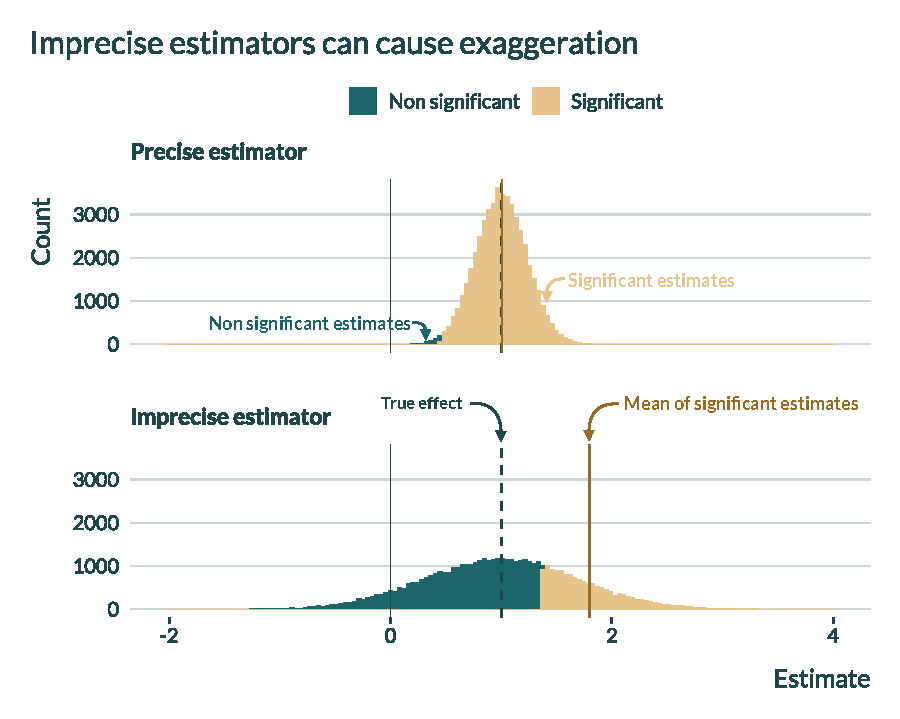
\includegraphics[width=0.8\linewidth]{images/graph_intuition_precision.pdf}
					\caption*{\footnotesize \textit{Notes}: 100,000 draws from two normal distributions $\mathcal{N}(1, 0.05)$ and $\mathcal{N}(1, 0.5)$.}
				\end{center}
				\vspace{-1cm}
			 \end{figure}
			
			Yet, exaggeration only arises when two circumstances are combined: 1) a publication bias favors statistically significant results and 2) statistical power is low. A large literature underlined the existence of the former in economics \citep[for instance]{rosenthal_file_1979, andrews_identification_2019, abadie_statistical_2020, brodeur_methods_2020}. Published estimates from under-powered studies thus form a biased sample of the distribution of estimates and can greatly exaggerate true effect sizes. Then, the economics literature, as others, suffers from a frequent and substantial lack of statistical power \citep{ioannidis_power_2017, ferraro_featureis_2020}. The resulting exaggeration has been documented as partly explaining the current replication failures observed in various fields such as economics, epidemiology, medicine or psychology \citep{button_power_2013, open_science_collaboration_estimating_2015, camerer_evaluating_2016, chang_is_2022}. Even in experimental economics, with a high level of control and an arguable absence of confounders, estimates published in top economic journals that have been replicated were on average inflated by a factor of at least 1.5 \citep{camerer_evaluating_2016}. Quasi-experimental studies are likely even more exposed to this exaggeration issue as, in current practices, statistical power is not central to such analyses. Several meta-analyses provide clear evidence of consequential exaggeration in the non-experimental economics literature. \cite{ioannidis_power_2017} finds that the median statistical power in a wide range of areas of economics is no more than 18\%. Despite the widespread use of convincing causal identification strategies and usually large sample sizes, they show that nearly 80\% of estimates are likely exaggerated by a factor of two. In environmental economics, \cite{ferraro_featureis_2020} finds that 56\% of estimates are exaggerated by a factor of two or more. In a companion paper, I document evidence of substantial exaggeration in a subfield of this literature, that on the acute health effects of air pollution \citep{bagilet_accurately_2023}. The magnitude of exaggeration is thus considerable and could in some situations be on par with that of a bias caused by confounders. 
			%Add CBA thing here
			It is thus crucial to take exaggeration into account and to understand its drivers.
			%In environmental economics, where estimates are often directly used to inform policies, in particular via CBA, obtaining accurate estimates is even more crucial. In this field, we often chase small and diffuse effects, that are intrinsically difficult to capture, often because playing a role in the long term or being causaly diffuse. 
			%It is even more important in some fields such as environmental economics where estimates are used to directly inform public policy. Via CBA 
			
			% goal of this study
			In this paper, I argue that the use of causal identification strategies contributes to exaggeration. %I propose an overarching mechanism that may contribute to do so. 
			Using a mathematical derivation and Monte Carlo simulations, I show that design choices in quasi-experimental studies can be seen as a trade-off between avoiding confounding and overestimating true effect sizes due to a resulting loss in power. To limit the threat of confounding, causal inference methods discard variation and therefore reduce statistical power. When combined with a statistical significance filter, this results in exaggeration bias. While causal identification strategies are essential to describe causal relationships, this paper emphasizes that a perfectly convincing identification does not guaranty an absence of ``bias'' and that improving identification can actually pull us away from the true effect. The same strategies which remove the bias caused by confounding factors actually introduce another type of bias.
			
			%mechanisms
			%I analyze the key factors affecting the confounding-exaggeration trade-off for a wide range of identification strategies : RD, IV, event studies, strategies such as DiD relying on  fixed effects (FEs) or generic controls and matching. 
			
			%IMPORTAAAAAANNNNTTT
			%Maybe change order
			All causal identification strategies discard variation in order to identify causal effects but the confounding-exaggeration trade-off is mediated through a distinctive channel for each of them. In RD designs, even when the initial sample size is large, we discard part of the variation by only considering observations within the bandwidth, decreasing the effective sample size and thus precision. In an IV setting, we only use the subset of the variation in the treatment that is explained by the instrument. In studies leveraging exogenous shocks, the variation used to identify an effect sometimes only comes from a limited number of changes in treatment status. Approaches that do not actually leverage natural experiments but aim to identify a causal effect by controlling for confounders also limit the variation used. 
			%When all confounders are arguably measured, matching has a causal interpretation but it still 
			Matching prunes units that cannot be matched and thus reduces the effective sample size. Adding controls or fixed effects to the model can increase the variance of the estimator and exaggeration if they absorb more of the variation in the treatment than in the outcome variable. 
			
			%IMPORTAAAAAANNNNTTT
			%I need to change and strengthen that: reorganize with the right id strats
			Since causal identification strategies can be interpreted as ways of controlling for confounders, this last point actually ties all the strategy-specific arguments together. We implement Fixed Effects (FEs) based identification strategies such as DiD to control for the invariant, unobserved, and arguably endogenous part of the variation in the outcome. In the Control Function (CF) approach to IV, we control for the variation in $x$ unexplained by the instruments. %the predicted residuals of the regression of the endogenous variable of interest on the instrument.
			 Fuzzy-RD and propensity score matching can also be thought of as control function approaches, of the forcing variable and propensity score respectively. In addition, excluding observations that are outside the bandwidth or unmatched is equivalent to controlling for observation-level fixed effects for these observations. When these methods for controlling for confounders absorb more of the variation in the treatment than in the outcome, they will increase the variance and cause exaggeration. Considering a simple linear homoskedastic model gives the intuition for this trade-off between exaggeration and omitted variable bias (OVB) for control approaches.  Let $y_{i} = \alpha + \beta x_{i} + \delta w_{i} + u_{i}$, $\forall i \in \{1, .., n\}$,  with $x$ the variable of interest, $w$ a potentially unobserved variable correlated with $x$ and $u$ an error term. Under usual assumptions and using the Frisch-Waugh-Lovell theorem, we get that $ \sigma_{\textsc{ovb}}^2$ and $ \sigma_{\textsc{ctrl}}^2$, the variance of the estimators for $\beta$ when omitting $w$ (short regression) and controlling for it (long regression) are respectively:
			~
			\[
				\sigma_{\textsc{ovb}}^2 =
				 \dfrac{\sigma^{2}_{u_{\textsc{ovb}}}}{n \ \sigma_{x}^{2}} =
				 \dfrac{\sigma^{2}_{y^{\perp x}}}{n \ \sigma_{x}^{2}}
				 \qquad \text{and} \qquad
				 \sigma_{\textsc{ctrl}}^2 = 
				 \dfrac{\sigma^{2}_{u_{\textsc{ctrl}}}}{n \ \sigma_{x^{\perp w}}^{2}} =
				  \dfrac{\sigma^{2}_{y^{\perp x, w}}}{n \ \sigma_{x^{\perp w}}^{2}}
			\]
			
			where $\sigma^{2}_{u_{\textsc{ovb}}}$ and $\sigma^{2}_{u_{\textsc{ctrl}}}$ are the variances of the residuals in the regression of $y$ on $x$ and of $y$ on $x$ and $w$ respectively, $\sigma^{2}_{y^{\perp x}}$ and $\sigma^{2}_{y^{\perp x, w}}$ are the variances of the parts of $y$ that are orthogonal to $x$ and to $x$ and $w$ respectively, $\sigma^{2}_{x}$ is the variance of $x$ and $\sigma^{2}_{x^{\perp w}}$ is the variance of the part of $x$ orthogonal to $w$. Thus,
			
			\[
				 \sigma_{\textsc{ctrl}}^2 > \sigma_{\textsc{ovb}}^2
				 	\quad \Leftrightarrow \quad 
				 	\dfrac{\sigma^{2}_{y^{\perp x, w}}}{n \ \sigma_{x^{\perp w}}^{2}} >
					\dfrac{\sigma^{2}_{y^{\perp x}}}{n \ \sigma_{x}^{2}} 
					\quad \Leftrightarrow \quad 
					\dfrac{\sigma^{2}_{y^{\perp x, w}}}{ \sigma_{y^{\perp x}}^{2}} >
					\dfrac{\sigma^{2}_{x^{\perp w}}}{\sigma_{x}^{2}}
			\]
			
			Controlling for $w$ will increase the variance of the estimator if the fraction of the variance unexplained by $w$ is greater for $y^{\perp x}$ than for $x$. Put differently, if controlling absorbs more of the variation in $x$ than in the residual part of $y$ ($y^{\perp x}$), it will increase the variance of the estimator. As briefly discussed above, since exaggeration increases with the variance of the estimator, controlling may increase exaggeration. I develop a formal proof showing that exaggeration can be larger when controlling, even when accounting for bias, in section \ref{maths}.
			
			% what we actually do
			In the remainder of the paper, I first derive a formal proof of the existence of the trade-off for prevailing causal identification strategies. Specifically, I show that the bias caused by exaggeration can be larger than the one caused by confounders. I also analyze the drivers of exaggeration and show that it increases as the strength of the instruments decreases, the number of exogenous shocks decreases or when controlling for a confounder absorbs more of the variation in the treatment than in the outcome. 
			
			 Then, I illustrate the existence of this ``causal exaggeration'' in realistic settings using examples drawn from environmental, education, labor, health and political economics. %We show that an actual trade-off between exaggeration and confounders can exist as exaggeration can be large for research designs implemented in actual studies. 
			The exaggeration of statistically significant estimates can be defined as the ratio of the estimated effect over the true effect, which is never known in a real world setting. I order to know the true effect and be able to compute this quantity, I turn to simulations. In addition, Monte-Carlo simulations allow to vary the value of the parameter of interest \textit{ceteris paribus}. An actual setting would for instance only allow to observe one strength for a given instrument. Since these simulations have an illustrative purpose only, I intentionally focus on settings in which statistical power can be low. All other simulation assumptions are chosen to make it as easy as possible to recover the effect of interest. I consider simple linear models with constant and homogenous treatment effects, \textit{i.i.d.} observations and homoskedastic errors. All the models are correctly specified and accurately represent the data generating process, except for the omitted variable.
									
			Finally, I discuss concrete avenues to address this causal exaggeration when carrying out a non-experimental study\footnote{In experimental studies, a solution to increase power is generally to increase sample size, reduce noise by improving measurement or improving balance or focus on larger potential effects.}. First, I advocate for the use of tools to evaluate the potential magnitude and risk of both confounding and exaggeration issues separately. Sensitivity analyses help with the former while power calculations help with the latter. %These power calculations can be computed before and after the analysis is carried out. 
			For instance, the sensitivity analysis tools developed in \cite{cinelli_making_2020} enable to assess how strong confounders would have to be to change the estimate of the treatment effect beyond a given level we are interested in. Then, considering the attention given to bias avoidance in the economics literature, I advocate to make power central to non-experimental analyses, even after an effect has been found, in order to limit bias caused by exaggeration. Prospective power simulations help identify the design parameters affecting power and exaggeration by approximating the data generating process \citep{gelman_regression_2020, black_simulated_2021}. Retrospective power calculations allow to evaluate whether a study would have enough power to confidently estimate a range of smaller but credible effect sizes \citep{gelman_beyond_2014, stommes_reliability_2021}.
			%%%%%%%% Evaluating potential exaggeration and confounders is however complex as both rely on unobserved shit
			Focusing more specifically on the trade-off and its drivers, I present tools to visualize the variation actually used for identification when using causal identification strategies. The \href{https://vincentbagilet.github.io/causal_exaggeration/}{companion website} describes in details how such analyses can be implemented. Finally, I briefly discuss potential solutions to mitigate this trade-off.
						
			% first contribution
			This paper contributes to three strands of the applied economics literature. First, the idea that causal identification estimators, while unbiased, may be imprecise is not new; this is part of the well-known bias-variance trade-off \citep{imbens_optimal_2012, deaton_understanding_2018, hernan_causal_2020, ravallion_should_2020}. I approach this literature from a different angle: through the prism of statistical power and publication bias. Not only the limited precision resulting from the use of causal identification methods could make it difficult to draw clear conclusions regarding the exact magnitude of the effect but I argue that it might also inherently lead to inflated published effect sizes, creating another ``bias''. The bias-variance trade-off can in fact be a bias-bias trade-off.
			
			% second contribution
			Second, studies discussing the exaggeration of statistically significant estimates due to a lack of power usually do not investigate its determinants and focus on specific causal identification methods separately \citep{ioannidis_power_2017, schell_evaluating_2018, ferraro_featureis_2020, black_simulated_2021, stommes_reliability_2021, young_leverage_2021}.  In a companion paper, I highlight tangible design parameters that can cause exaggeration for a wide range of empirical designs \citep{bagilet_accurately_2023}. In the present paper, I take a step back and propose an overarching mechanism, inherent to causal identification strategies as a whole, and that can explain these issues: although each strategy does so through different means, in essence they discard part of the variation, thereby increasing the risks of exaggeration. %This connection could be exacerbated by the fact that, as noted by \cite{brodeur_methods_2020}, publication bias is more prevalent for some methods such as the IV. 
			
			% third contribution
			Third, this study contributes to the literature on replicability in economics \citep{camerer_evaluating_2016, ioannidis_power_2017, christensen_transparency_2018, kasy_forking_2021}. The trade-off presented in this paper suggests that the widespread use of convincing causal identification methods in economics may not shield the field from potential replication threats.
			%The trade-off presented in this paper may contribute to explaining the replication failures observed in empirical economics, despite the widespread use of convincing causal identification methods.
			
			In the following section, I study the drivers of exaggeration and formally show in a simple setting that the use of causal identification strategies can exacerbate it. In section  \ref{simulations}, I implement realistic Monte-Carlo simulations to illustrate the existence of the confounding-exaggeration trade-off. I discuss potential solutions to navigate this trade-off in section \ref{discussion} and conclude in section \ref{conclusion}.
	
	
		
	
%-----------------------------------------------------------------------------

% LIT REVIEW

%-----------------------------------------------------------------------------

	\section{Causal Exaggeration in the Literature}\label{lit_review}
	
		The trade-off presented in this paper has meaningful implications only if causal identification strategies lead to substantial exaggeration, especially as compared to the amount of confounding bias they allow avoiding. This section aims to documents the existence of such exaggeration in the causal economics literature. 
		
		A first piece of evidence emerges from the observation that causal methods routinely yield larger estimates than association-based approaches. The data in \cite{young_consistency_2022} reveals that among 30 reproducible papers published in journals from the  \textit{American Economic Association}\footnote{The exact selection process is described in section 3 of \cite{young_consistency_2022}. The sample consists of papers using the keyword ``instrument'', published up through July 2016, that are reproducible, relying on open access data and Stata code, using linear methods and standard covariance estimates.}, the median ratio of headline IV estimates over the corresponding OLS is 2.3, with 25\% of estimates exceeding a ratio of 5.4. A comparable pattern appears in top political science journals \citep{lalHow2024}. In the literature on the acute health effects of air pollution, which I explore in a companion paper, causal estimates are substantially larger than what would have been predicted by the standard epidemiology literature, estimates being regularly more than 10 times larger \citep{bagilet_accurate_2023}. Even within a given setting and study, the median of the ratio of the obtained 2SLS to their corresponding ``naive'' OLS estimates is 3.8. 
		
		What can explain that causal methods yield such large effects sizes, as compared to non-causal methods? They could arguably remove omitted variable bias, reduce attenuation bias caused by classical measurement error or target a different causal estimand. But as I argue in this section, exaggeration and imprecision could also explain part of this difference. For instance, published IV papers typically have low power and make most 2SLS estimates statistically indistinguishable from the corresponding OLS \citep{young_consistency_2022}. %In the example case of studies on the short-term health effects of air pollution, causal studies often display a low relative precision, not only because effects are typically small and the data relatively coarse---at the city-day level---but also because they sometimes leverage rare exogenous shocks such as public transportation strikes, take advantage of air pollution alerts to build RDD that limit sample size or use instruments that do not strongly predict air pollution levels \citep{bagilet_accurate_2023}.
				 
%		 On the other hand, in some settings, bias caused by confounders may not be as large. 
%			For instance, \cite{young_consistency_2022} shows that in instrumental variables papers published in journals from the American Economic Association a lack of precision makes most of the 2SLS estimates statistically indistinguishable from the corresponding OLS. \cite{weidmann_lurking_2021} documents an absence of evidence of selection bias due to unobservables in the evaluations of school programs they investigate.
%		 In situations where confounding bias is limited but the loss in statistical power resulting from the use of a causal method likely large, a traditionally biased but more precise method may lead to less overall bias, accounting for exaggeration. Regardless, the bias resulting from the use of causal methods, even 
		 
	                \subsection{Quantifying exaggeration}
	                
	                	 	As discussed in the introduction, lack of power is widespread and exaggeration substantial in the economics literature; \cite{ioannidis_power_2017} estimates that nearly 80\% of results published in a wide array of empirical economic literatures are likely exaggerated, typically by a factor of two and one-third by a factor of four or more. %In environmental economics, using a more conservative approach, \cite{ferraro_featureis_2020} estimates that 56\% of results are exaggerated by a factor of two or more.
			
				To document exaggeration in the causal inference literature more specifically, and to compute exaggeration in general, one needs to  hypothesize true effect sizes. I begin by examining broad literatures that in return require strong assumptions about true effect sizes, then progressively narrow my focus to more specific literatures that allow these assumptions to be relaxed. I first leverage data from \cite{brodeur_methods_2020}. This paper reviews of the universe of hypothesis tests reported in papers published in the top-25 economics journals in 2015 and 2018 and using RCT, DID, RDD or IV. It shows that IV and to a lesser extent DID are particularly subject to publication bias---one of the two ingredients of exaggeration. 
			Since the exaggeration ratio is the expected value of the absolute value of significant estimates over the true effect, it can only be calculated by hypothesizing true effect sizes. 
			%Considering the wide variety of treatments and outcomes in the literature on the acute health effects of air pollution, there is a multitude of estimands and ``true effects''. 
			To circumvent this limitation, I first evaluate the proportion of studies in \cite{brodeur_methods_2020} that would have a design reliable enough to retrieve an effect size equal to half of the obtained estimate. I also compute the exaggeration of significant estimates under this hypothesis. There is no \textit{a priori} reason to believe that the magnitude of the true effect of a specific estimation would be equal to half its point estimate. However, since \cite{ioannidis_power_2017} finds a typical exaggeration of two in the economics literature, we may expect this assumption to be reasonable, on average. Regardless, I do not claim that the true effect is equal to this hypothesized value but rather wonder what would be the power and exaggeration under this justifiable assumption. This approach is also to some extent conservative: hypothesized effect sizes based on exaggerated estimates will be larger and will thus minimize exaggeration.
			
			 The exaggeration is computed by drawing a large number of times from a normal distribution centred on the hypothetical effect size and with a standard deviation equal to the standard error of the estimate found in the study and by then computing the average of the draws that are 1.96 standard errors away from 0. I further discuss how to compute such power calculations in section \ref{retro_calc}. Under this assumption regarding the effect size, the median power and median exaggeration ratio of significant estimates in the data from \cite{brodeur_methods_2020} would be 37\% and 1.6 respectively. Statistical power would be larger than the usual 80\% threshold for only 22\% of designs. 28\% of the designs would, on average, exaggerate the true effect sizes by more than a factor of 2. While exaggeration is reassuringly limited in some settings, it can be substantial in many others. These results are relatively comparable across methods (IV, DID, RDD and RCT). 
			
			While the previous hypothesis regarding true effect sizes provides a broad overview of the literature, it may seem somewhat arbitrary. To reduce the burden of assumptions, I narrow the focus to IV designs, which enable a more systematic intra-study comparison between the 2SLS estimates and the corresponding ``naive'' OLS one. I do not claim that the OLS estimate accurately represents the true effect but it may be reasonable to expect the IV to have enough power to retrieve an effect of the magnitude of the OLS point estimate, if it was indeed the true effect. To explore this question, I leverage the data from \cite{young_consistency_2022}. IV designs that produced significant headline results would only have a median power of 25\% to detect an effect size of the magnitude of the OLS estimate. Significant estimates from half of these designs would exaggerate the OLS estimate by a factor larger than 2 and a quarter would do so by a factor larger than 3.5. Only 17\% of these designs would reach the conventional 80\% power threshold. These figures further underline heterogeneity in vulnerability to exaggeration and power issues. While many analyses are likely immune to exaggeration, a substantial share of them would not be powered enough to detect effects of realistic magnitude leading significant estimates to considerably exaggerate these effects.\footnote{I find similar results in the literature on acute health effects of air pollution and in the political science literature, leveraging reviews implemented in \cite{bagilet_accurate_2023} and \cite{lalHow2024} respectively. The experimental literature displays less exaggeration on average but still substantial heterogeneity \cite{camerer_evaluating_2016}. These analyses are described on \href{https://vincentbagilet.github.io/causal_exaggeration/lit_IVs.html}{the project's website}.} These results complement the analysis in \cite{young_consistency_2022} that highlights the imprecision of published 2SLS estimates, making them statistically indistinguishable from the corresponding OLS estimate, despite the fact that 2SLS point estimates substantially differ in magnitude from their OLS counterpart and are even regularly  of the opposite sign. %In the literature on the short-term health effects of air pollution, the median power of the 2SLS to retrieve an effect of the same magnitude as the OLS would only be 12\% and median exaggeration would reach 4.5. 
			
	\subsection{Illustration of the trade-off}
	
		In order to limit hypotheses and to investigate causal exaggeration further, I focus on an example IV study investigating the impact of PM2.5 air pollution on mortality \citep{he_straw_2020}. It allows comparing the bias of the ``naive'' OLS to that of the IV by computing their distance to an estimate of the ``true effect'' they target. %\footnote{I am currently carrying out the same analysis for other studies. However, variation in the treatments and outcome considered make comparisons challenging. In addition, the number of existing studies that correspond to the necessary criteria is limited (16). Computing summary statistics on such a small sample may be irrelevant, especially since the risk of exaggeration varies a lot across these studies. I thus plan to display results study by study.} %When the IV estimate differs from this ``true effect'', I explore whether exaggeration could explain this difference.
		%The ``true effect'' is the central piece of the analysis. 
		I define this ``true effect'' in two ways. First, I use the results of a meta-analysis of epidemiological studies \citep{shah_short_2015}. By pooling a number of studies carried out in various contexts, this meta-estimate might represent the average effect one may expect from such a study.  However, the studies in this meta-analysis do not rely on canonical causal identification strategies used in economics and may be thought of as suffering from counfounding. I thus consider the result of \cite{deryugina_mortality_2019}---a precise causal study that may be less exposed to exaggeration---as an alternative estimate of the ``true effect''. This estimate may be context specific and the ``true effect'' in %a particular study 
		\cite{he_straw_2020} may deviate from these. 
		The present discussion is conditional on this true underlying effect being close to these hypothesized true effect sizes.\\
		
		\cite{he_straw_2020} finds that a ``$10 \mu g.m^{-3}$ increase in PM2.5 increases mortality by 3.25\%'' (s.e. 1.43\%). Their corresponding OLS results suggest a 0.32\% increase (s.e. 0.23\%). 
For a similar increment in air pollution, \cite{shah_short_2015} and \cite{deryugina_mortality_2019} document a 1.1\% and 1.8\% increase in mortality respectively. The OLS estimate in \cite{he_straw_2020} is closer to the ``true effect'' based on \cite{shah_short_2015} than their 2SLS estimate. Provided that the three estimands are comparable, the bias of the IV is larger than that of the OLS. If the true effect was in fact closer to the one found by \cite{deryugina_mortality_2019}, both biases would be roughly equal and the bias of the IV still substantial.
		
		Exaggeration could explain this difference. Even if the 2SLS estimator effectively removes all conventional biases, the design in \cite{he_straw_2020} would still yield exaggerated statistically significant estimates. Figure \ref{graph_he} illustrates this point. Even if the 2SLS estimator is unbiased, i.e., centered on the meta-estimate found in \cite{shah_short_2015}, the lack of precision of this design would lead significant estimates to substantially exaggerate the true effect, by a factor 3.2 on average.  The 2SLS estimate found in \cite{he_straw_2020} could be one of these estimates.
				
		\begin{figure}[!h]
                   	\caption{Illustration of the Confounding-Exaggeration Trade-off in \cite{he_straw_2020}}
                        \label{graph_he}
                    	\centering
                    	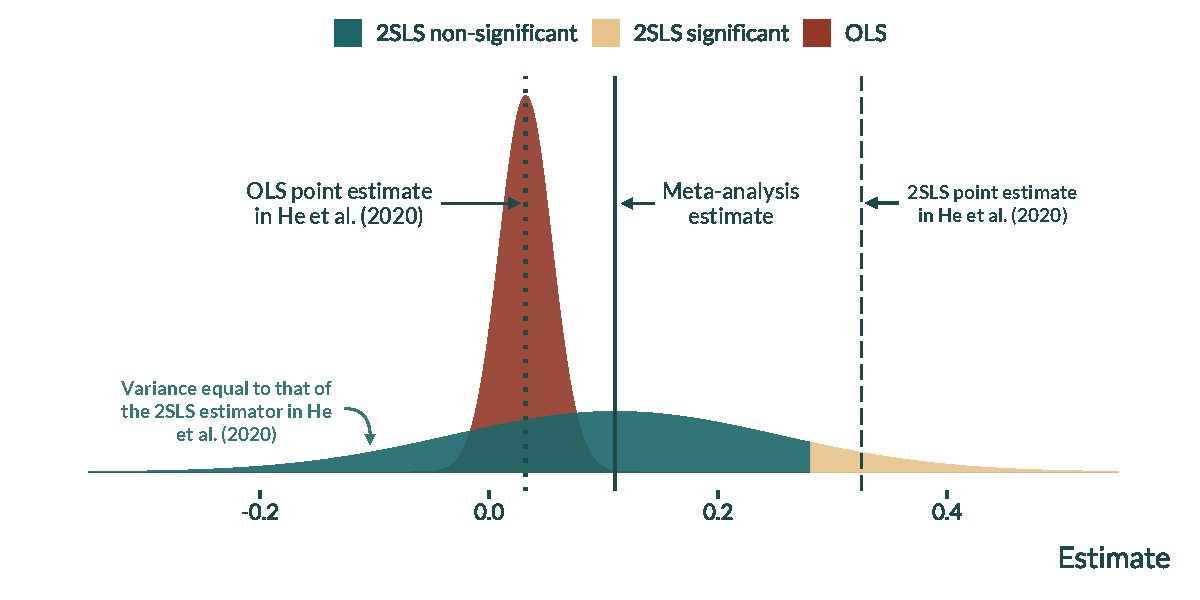
\includegraphics[width=0.85\linewidth]{images/graph_he_th_annotated.pdf}
                   	 \caption*{\footnotesize \textnormal{\textit{Notes}:  %10000 draws from two normal distibutions. 
	 The distribution for the 2SLS estimator is centered on the true effect, represented by the solid line and defined as the meta-estimate found in \cite{shah_short_2015}. Its variance is equal to the one of the 2SLS estimator in \cite{he_straw_2020}. The distribution for the OLS estimator is centered on the OLS estimate found in \cite{he_straw_2020} and its variance equal to that of this same estimator. The dashed and dotted lines represent the 2SLS and OLS estimates found in \cite{he_straw_2020} respectively. I ignore exaggeration of the OLS for clarity but since the OLS is biased downward, inflating OLS estimates bring them closer to the true effect. }}
                \end{figure}
						
		This example illustrates that in a published study where a causal identification strategy substantially reduces the precision of the estimator, the resulting statistically significant estimates may be further away from the true effect than the ``naive'' OLS estimate, even if the estimator is unbiased. Note that a comparable result holds if the true effect is equal to the one found in \cite{deryugina_mortality_2019}. With this design, the average exaggeration would be 3.1 times larger than the OVB (or 1.3 time if the true effect is closer to the one found in \cite{deryugina_mortality_2019}).


%-----------------------------------------------------------------------------

% MATHS

%-----------------------------------------------------------------------------
	
	\section{Mathematical derivation} \label{maths}
						
		In this section, I formally prove the existence of the confounding-exaggeration trade-off  and describe its drivers in a simple setting. %\footnote{A more detailed version of this mathematical derivation is available on the \href{https://vincentbagilet.github.io/causal_exaggeration/Maths/math_causal_exaggeration.pdf}{companion website}.} 
		To do so, I first define an exaggeration ratio  and show that it increases with the variance of normally distributed biased estimators. I then compute the asymptotic distributions of a series of estimators and study drivers of their variances, and ultimately of their exaggeration ratios. Finally, I show that, for any magnitude of OVB, exaggeration can be greater when using a causal inference method than the overall bias combining exaggeration and OVB in the naive regression.
		
%%%%%%%%%%%%%%  Exagg ratio  %%%%%%%%%%%%%%%%%%%%%%%%%%%%%
		
		\subsection{Properties of the exaggeration ratio}\label{general_exagg}
		
			Following  \cite{gelman_beyond_2014}, we can define the exaggeration ratio $E$, as the expectation of the absolute value of significant estimates over the absolute value of the true effect. For an estimator $\hat{\beta}$ of a true effect $\beta$, with standard error $\sigma$ and a two-sided hypothesis test of size $\alpha$ with threshold value $z_{\alpha}$, let
			
			%Let's define an exaggeration ratio $E$, as the expected value of significant estimates over the true effect\footnote{Note that \cite{gelman_beyond_2014} define exaggeration as the expected value of the \textit{absolute value} of the estimate: $\mathbb{E}[ | \hat{\beta}| | \beta, \sigma, | \hat{\beta} | > z_{\alpha} \sigma ] / | \beta |$. Problematically, this expression, when not conditioning on significance, \textit{i.e.} $\mathbb{E}[ | \hat{\beta}| | \beta, \sigma ] / | \beta |$, is not equal to 1 for unbiased estimators, if statistical power is low. The alternative definition I use satisfies this key condition. My exaggeration ratio is also smaller or equal to \citeauthor{gelman_beyond_2014}'s and thus more conservative.}. Formally, we have:
		 
				 \begin{equation}\label{exagg_general}
				 	E(\hat{\beta}, \sigma, \beta, z_{\alpha}) =
					 	\dfrac{\mathbb{E}\left[ | \hat{\beta} | \big| \beta, \sigma, |\hat{\beta}| > z_{\alpha} \sigma \right]}{| \beta |} 
				\end{equation}
				
			\cite{lu_note_2019} and \cite{zwet_significance_2021} showed that, for given test and true effect sizes, the exaggeration ratio increases with the variance of an unbiased normally distributed estimator. We can extend this proof to biased estimators and get that:\footnote{All the proofs of the lemma and theorems are reported in appendix \ref{maths_proofs}.}
			
			\begin{lemma}
				\label{lemma_drivers}
			
				For an estimator $\hat{\beta_{b}}  \sim \mathcal{N}(\beta + b, \sigma^{2})$ of a true effect of magnitude $\beta$ and a fixed bias $b$ of the same sign as and independent from the true effect,
				
				\begin{itemize}
					\item $E$ is a decreasing function of the Signal-to-Noise Ratio (SNR) $\frac{\beta}{\sigma}$, \textit{ie} the relative precision of the estimator, and only depends on $\sigma$ through this SNR. 
					\item  $\lim_{\sigma\to \infty} E(\hat{\beta_{b}}, \sigma, \beta, z_{\alpha}) = +\infty$.
				\end{itemize}
			\end{lemma}
			
				Figure \ref{fig:graph_exag} provides a clear intuition for these results in the unbiased case. Note that here, we conservatively focus on cases in which the bias is in the same direction as the true effect so that exaggeration from causal inference methods and OVB do not cancel each other.\\
				 
				 Based on lemma \ref{lemma_drivers}, one only needs to show asymptotic normality and study how the variances of these estimators evolve with these parameters to study how exaggeration evolves with the IV strength in an IV setting, the number of exogenous shocks in a reduced form and the correlation between the explanatory variable of interest and the omitted variable of interest. This relies on the assumption that the sample size is large enough so that the sample distribution of the estimator is well approximated by their asymptotic distribution.
				 				 
		\subsection{Setting and data generating process}\label{maths_dgp}
		
			Consider a usual linear homoskedastic regression model with an omitted variable. For any individual $i \in \{1, ..., n\}$, we write:
				~
				\begin{equation}\label{maths_dgp_y}
					y_i = \beta_{0} + \beta_{1}x_{i} + \delta w_{i} + u_i
				\end{equation}
				
				where $y$ is the outcome, $x$ the explanatory variable,  $w$ an unobserved omitted variable, $u$ an unobserved error term.  $(\beta_0, \beta_1, \delta) \in \mathbb{R}^{3}$ are unknown parameters. $\beta_1$ is the parameter of interest.\\
			
			Assume homogeneous treatment effects and homoskedasticity, along with the usual OLS assumptions (\textit{i.i.d.} observations, finite second moments, positive-definiteness of $\mathbb{E}[\text{x}_i \text{x}_i']$---with $\text{x}_i = (1, x_i)'$--- and $u_{i}$ conditional mean-zero and uncorrelated with $x_i$ and $w_i$). Assume that $w_{i}$ is unobserved, correlated with $x_{i}$ and that $\delta \neq 0$. To simplify the derivations, I further assume that the unobserved variable is centered, \textit{i.e.} $\mathbb{E}[w_i] = 0$. I also assume that the variance of the component of $w_{i}$ that is orthogonal to $x_{i}$ (denoted $w_{i}^{\perp x}$) does not vary with $x_{i}$, \textit{i.e.}, $\text{Var}(w_{i}^{\perp x}|x_{i}) = \text{Var}(w_{i}^{\perp x})$. Consider the following data generating process for $x_i$:
				~
				\begin{equation}\label{maths_dgp_x}
					x_i = \mu_{x} + \gamma w_{i} + \epsilon_i
				\end{equation}
				
				where $\gamma \in \mathbb{R}^{*}$ since $x$ and $w$ are correlated. Set $\rho_{xw} = \text{corr}(x, w) =  \frac{\gamma \sigma_{w}}{\sigma_{x}}$. In the IV and reduced form sections, I further assume that there exists a valid instrumental variable $z_i$ for $x_i$, \textit{i.e.} that $\mu_x + \epsilon_{i} = \pi_0 + \pi_1 z_i + e_{i}$  where $(\pi_0, \pi_1) \in \mathbb{R}^{2}$ are unknown parameters. The existence or not of this valid instrument does not affect the results in the controlled and \textsc{OVB} cases. Since the instrument is valid, it satisfies exogeneity, \textit{i.e.} $\mathbb{E}[\text{z}_{i}u_{i}] = 0$ and  $\mathbb{E}[z_{i}w_{i}] = 0$, relevance, \textit{i.e.} $\text{rank}(\mathbb{E}[\text{z}_{i}\text{x}_i']) = 2$,  and positive-definiteness of $\mathbb{E}[\text{z}_i \text{z}_i']$. The data generating process for $x_i$ becomes:			
				~
				\begin{equation}\label{maths_dgp_x_iv}
					x_i = \pi_0 + \pi_1 z_i + \gamma w_{i} + e_{i}
				\end{equation}
				
				I assume that $e_{i}$ is uncorrelated with $z_i$ and $w_{i}$, \textit{i.e.} $\mathbb{E}[z_ie_{i}] = 0$ and $\mathbb{E}[w_ie_{i}] = 0$. I also assume homoskedasticity for this term, such that $\mathbb{E}[e_{i}^{2} | z_{i}, w_{i}] = \sigma_{e}^{2}$ is constant.\\ %It implies that  $\mathbb{E}[e_{i}^{2} | z_{i}] = \sigma_{e}^{2}$ (since $\mathbb{E}[e_{i}^{2} | z_{i}] =  \mathbb{E}[\mathbb{E}[e_{i}^{2} | z_{i}, w_{i}] | z_{i}] = \mathbb{E}[\sigma_{e}^{2} | z_{i}] = \sigma_{e}^{2})$.\\
				
				Overall, this DGP is close to the usual textbook one but with an additional omitted variable. The Directed Acyclic Graph (DAG) in figure \ref{DAG} represents the data generating process.
			
			 \begin{figure}[!h] 
                    			\begin{center}
                    				\caption{DAG of the data generating process}
                    				\label{DAG}
                    				\includegraphics[width=0.6\linewidth]{images/DAG_maths.png}
                                   \caption*{\footnotesize \textit{Notes}: for clarity the error terms are represented in this graph, in beige. Model parameters are noted as edge labels.}
                                    \end{center}
				\vspace{-1cm}
                    		\end{figure} 

				
%%%%%%%%%%%%  ASYMPTOTIC DISTRIB  %%%%%%%%%%%%%%%%%%%%%%%%
		
		\subsection{Asymptotic distributions of the estimators}\label{maths_asymptotics}			 
			
			I now derive the asymptotic distributions of the various estimators. For each model, the goal is to show asymptotic normality and to study the evolution of the sampling distribution variances with the value of the parameter of interest, \textit{i.e.}, a measure of the correlation between $x$ and $w$ ($\gamma$) in the controlled case, of the IV strength ($\pi_{1}$) in the IV case and of the number of exogenous shocks ($\sigma_{z}^{2}$ when $z$ is a dummy) in the reduced form case. I assume that the sampling distributions are well approximated by the asymptotic distributions. %Since variables and parameters are intertwined, modifying the value of one of them can affect the value of the others. 
			In order for the variation of one factor not to impact other factors of interest, I consider the variances of the variables ($\sigma_{y}^{2}, \sigma_{x}^{2}, \sigma_{w}^{2} \text{ and } \sigma_{z}^{2}$) as fixed but adjust for the variances of the error terms ($\sigma_{u}^{2} \text{ and } \sigma_{\epsilon}^{2}$) when varying the values of one of the parameters ($\gamma, \delta \text{ and } \pi_{1}$). This corresponds to thinking in terms of shares of the variance of $x$ and $y$ explained by ``defined'' variables (\textit{i.e.}, observed variables and $w$) \textit{versus} by residuals. Finally note that comparison between cases with and without OVB for different parameter values is only relevant if varying the parameter of interest does not affect the OVB. I thus make comparative statics analyses at bias fixed, \textit{i.e.}, as shown below, for $\gamma \delta = \kappa = cst$.
			
%%%%%%%%%%%%%%  OVB  %%%%%%%%%%%%%%%%%%%%%%%%%%%%%

			\subsubsection{Naive regression (OVB)}\label{formal_proof_ovb}
			
%				First, consider a ``naive'' regression of $y$ on $x$ (with $w$ omitted). The formula for the bias can easily computed using textbook algebra. The intuition for the formula of the main parameter of interest, the asymptotic variance, has been discussed in the introduction: as in the standard case, the variance of the estimator is given by the ratio of the variance in $y$ that is not explained by $x$ ($\sigma^{2}_{y^{\perp x}}$), over the variance of $x$ multiplied by the number of observations. The only difference with the standard case is the presence of the omitted variable $w$. From equation \ref{maths_dgp_y}, it is clear that $\sigma^{2}_{y^{\perp x}} = \sigma^{2}_{u^{\perp x}} + \delta^{2}\sigma^{2}_{w^{\perp x}}$. A more rigorous derivation described in appendix \ref{maths_proofs} leads to the following lemma:
%				%Since, $w$ is unobserved, we consider the projection of $y$ on $X$ only, where $X = (\text{x}_{1}', ..., \text{x}_{n}')'$ with $\forall i, \text{x}_{i}' = (1, x_{i})$
%%					~
%%					\begin{equation}\label{maths_eq_ovb}
%%						y = X\bm{\beta}_{\textsc{ovb}} + u_{\textsc{ovb}}
%%					\end{equation}
%%				
%%				with, by definition of the projection, $\mathbb{E}[X'u_{\textsc{ovb}}] = 0$.
%						
%				\begin{lemma}\label{lemma_ovb}
%					Based on the data generating process described in section \ref{maths_dgp}, for $\hat{\beta}_{\textsc{ovb}}$ the OLS estimate of $\beta_{1}$ in the regression of $y$ on $x$, $\hat{\beta}_{\textsc{ovb}} \overset{d}{\to} \mathcal{N}(\beta_{1} + b_{\textsc{ovb}} , \ \sigma_{\textsc{ovb}}^{2})$, with
%					\[
%						b_{\textsc{ovb}} = \dfrac{\delta \gamma \sigma_{w}^{2}}{\sigma_{x}^{2}} 
%						\qquad \text{and} \qquad
%						\sigma_{\textsc{ovb}}^{2} = \dfrac{\sigma_{u}^{2} + \delta^{2} \sigma_{w}^{2}(1 - \rho_{xw}^{2})}{n \ \sigma_{x}^{2}}
%						%\sqrt{n}\left( \hat{\beta}_{\textsc{ovb}} - \left(\beta_{1} + \dfrac{\delta \gamma \sigma_{w}^{2}}{\sigma_{x}^{2}}\right) \right)
%						 %\overset{d}{\to} \mathcal{N}\left( 0 , \ \dfrac{ \sigma_{u}^{2} +  \delta^{2} \sigma_{w}^{2} (1 - \rho_{xw}^{2} )}{\sigma_{x}^{2}} \right) 
%					\]
%				\end{lemma}
%				
%			Note that since $\sigma_{x}^{2}$ and $\sigma_{w}^{2}$ are fixed, reasoning at $b_{\textsc{ovb}} = cst$ is equivalent to considering that $\gamma \delta = \kappa = cst$. Then, noting that $\forall i, u_{i} = y_i - \beta_{0} - \beta_{1}x_{i} - \delta w_{i}$ and computing its variance, we can rewrite the variance of the estimator as a function of fixed variances and one or less varying parameter:
			
				First, let us study the benchmark against which we are going to compare our causal approaches. Consider the ``naive'' regression of $y$ on $x$ (with $w$ omitted). 
				%Since, $w$ is unobserved, we consider the projection of $y$ on $X$ only, where $X = (\text{x}_{1}', ..., \text{x}_{n}')'$ with $\forall i, \text{x}_{i}' = (1, x_{i})$
%					~
%					\begin{equation}\label{maths_eq_ovb}
%						y = X\bm{\beta}_{\textsc{ovb}} + u_{\textsc{ovb}}
%					\end{equation}
%				
%				with, by definition of the projection, $\mathbb{E}[X'u_{\textsc{ovb}}] = 0$.
						
				\begin{lemma}\label{lemma_ovb}
					Based on the data generating process described in section \ref{maths_dgp}, for $\hat{\beta}_{\textsc{ovb}}$ the OLS estimate of $\beta_{1}$ in the regression of $y$ on $x$, $\hat{\beta}_{\textsc{ovb}} \overset{d}{\to} \mathcal{N}(\beta_{1} + b_{\textsc{ovb}} , \ \sigma_{\textsc{ovb}}^{2})$, with
					\[
						b_{\textsc{ovb}} = \dfrac{\delta \gamma \sigma_{w}^{2}}{\sigma_{x}^{2}} 
						\qquad \text{and} \qquad
						\sigma_{\textsc{ovb}}^{2} = \dfrac{\sigma_{u}^{2} + \delta^{2} \sigma_{w}^{2}(1 - \rho_{xw}^{2})}{n \ \sigma_{x}^{2}}
						%\sqrt{n}\left( \hat{\beta}_{\textsc{ovb}} - \left(\beta_{1} + \dfrac{\delta \gamma \sigma_{w}^{2}}{\sigma_{x}^{2}}\right) \right)
						 %\overset{d}{\to} \mathcal{N}\left( 0 , \ \dfrac{ \sigma_{u}^{2} +  \delta^{2} \sigma_{w}^{2} (1 - \rho_{xw}^{2} )}{\sigma_{x}^{2}} \right) 
					\]
				\end{lemma}
				
			The intuition for the formula of the asymptotic variance has been discussed in the introduction: $\sigma_{u}^{2} + \delta^{2} \sigma_{w}(1 - \rho_{xw}^{2})$ is the part of the variance in $y$ that is not explained by $x$ ($\sigma^{2}_{y^{\perp x}}$).\\
			
			Varying the parameter of interest, $\rho_{xw}$, will change the bias and $\sigma_{u}^{2}$. Since $\sigma_{x}^{2}$ and $\sigma_{w}^{2}$ are fixed, reasoning at $b_{\textsc{ovb}} = cst$ is equivalent to considering that $\gamma \delta = \kappa = const$. Then, noting that $\forall i, u_{i} = y_i - \beta_{0} - \beta_{1}x_{i} - \delta w_{i}$ and computing its variance, we can rewrite the variance of the estimator as a function of fixed variances and one or less varying parameter:
			~
			\[
				\sigma_{\textsc{ovb}}^{2} = \dfrac{\sigma_{y}^{2} - \beta_{1}^{2}\sigma_{x}^{2} - 2\beta_{1}\kappa\sigma_{w}^{2} - \kappa^{2}\frac{\sigma_{w}^{4}}{\sigma_{x}^{2}}}{n \ \sigma_{x}^{2}}
			\]
			
			 This expression underlines that, for a given bias,  $\sigma_{\textsc{ovb}}^{2}$ does not vary with $\gamma$, or equivalently $\delta$, the parameters of interest. Applying lemma \ref{lemma_drivers} proves that $E_{\textsc{ovb}}$ does not either.

%%%%%%%%%%%%%%  CTRL  %%%%%%%%%%%%%%%%%%%%%%%%%%%%%
			
			\subsubsection{Controlled regression}
			
				Next, let us turn to the ``ideal'' case in which no variable is omitted, \textit{i.e.} we control for the omitted variable $w$ and thus partial out confounders. The model considered accurately represents the DGP.
%				~
%				\begin{equation}\label{maths_eq_ovb}
%					y = X_{w}\bm{\beta}_{\textsc{ctrl}} + u_{\textsc{ctrl}}
%				\end{equation}
%				
				%with $X_{w} = (\text{x}_{w, 1}', ..., \text{x}_{w, n}')'$ with $\forall i, \text{x}_{w, i}' = (1, x_{i}, w_{i})$ and $\mathbb{E}[X_{w}'u] = 0$. 
				This corresponds to the usual OLS setting with a constant and two regressors that are uncorrelated with the error: $y$ regressed on $x$ and $w$.
						
				\begin{lemma}\label{lemma_ctrl}
					Based on the data generating process mentioned previously, for $\hat{\beta}_{\textsc{ctrl}}$ the OLS estimator of $\beta_{1}$ in the regression of $y$ on $x$ and $w$, $\hat{\beta}_{\textsc{ctrl}} \overset{d}{\to} \mathcal{N}(\beta_{1}, \ \sigma_{\textsc{ctrl}}^{2})$, with
					\[
						\sigma_{\textsc{ctrl}}^{2} = \dfrac{\sigma_{u}^{2}}{n \ \sigma_{x}^{2} (1 - \rho_{xw}^{2})}
					\]
				\end{lemma}
				
				$\sigma_{x}^{2} (1 - \rho_{xw}^{2})$ is the part of the variance of $x$ that is not explained by $w$ ($\sigma^{2}_{x^{\perp w}}$) and $\sigma_{u}^{2}$ the part of the variance of $y$ that is not explained by $x$ nor $w$ ($\sigma^{2}_{y^{\perp x, w}}$); here too we retrieved a result described in introduction. For a given bias, we then rewrite $\sigma_{\textsc{ctrl}}^{2}$ as a function of fixed variances and one varying parameter, $\gamma$:
				~
				\[
					\sigma_{\textsc{ctrl}}^{2} = \dfrac{\sigma_{y}^{2} - \beta_{1}^{2}\sigma_{x}^{2} - \frac{\kappa^{2}}{\gamma^{2}}\sigma_{w}^{2} - 2\beta_{1}\kappa \sigma_{w}^{2}}{n \ (\sigma_{x}^{2}  - \gamma^{2} \sigma_{w}^{2})}
				\]
				
				Since the numerator and denominator respectively increase and decrease with $|\gamma|$,  $\sigma_{\textsc{ctrl}}^{2}$ increases with $|\gamma|$. For a given bias, the more $w$ is correlated with $x$ (and thus roughly the less it is with $y$ since $\delta \gamma = const$), the larger the variance of the estimator. In addition, we can note that, for a given bias, the variance of the estimator can be arbitrarily large since $\lim_{\gamma^{2} \to \frac{\sigma_{x}^{2}}{\sigma_{w}^{2}}} \sigma_{\textsc{ctrl}}^{2} = + \infty$.
				
			
%%%%%%%%%%%%%%  IV   %%%%%%%%%%%%%%%%%%%%%%%%%%%%%	
		
		\subsubsection{Instrumental Variables}
		
			In the previous section, we considered a case in which we removed variation that included unwanted endogenous variation. We now turn to the IV, a converse situation where we select variation we want, exogenous variation. We estimate the IV model in which we regress $y$ on $\text{x}_{i} = (1, x_{i})'$ instrumented by $\text{z}_{i} = (1, z_{i})'$. We are thus in a just-identified case and $\hat{\bm{\beta}}_{\textsc{2sls}} = \hat{\bm{\beta}}_{\textsc{iv}}$.						
			\begin{lemma}\label{lemma_iv}
				Based on the data generating process mentioned above, for $\hat{\beta}_{\textsc{iv}}$ the IV estimator of $\beta_{1}$ in the regression of $y$ on $x$ instrumented by $z$,  $\hat{\beta}_{\textsc{iv}} \overset{d}{\to} \mathcal{N}(\beta_{1}, \ \sigma_{\textsc{iv}}^{2})$, with
					\[
						\sigma_{\textsc{iv}}^{2} = \dfrac{\sigma_{u}^{2} + \delta^{2}\sigma_{w}^{2}}{n \ \sigma_{x}^{2} \rho_{xz}^{2}}
					\]
			\end{lemma}
			
			The numerator is $\sigma_{y \perp \hat{x}}^{2}$, the part of the variance in $y$ that is not explained by $\hat{x}$, the predicted value of $x$ in the first stage and the denominator is $\sigma_{\hat{x}}^{2}$. For a given bias, noting that $\rho_{xz} = \text{corr}(x, z) = \pi_1 \frac{\sigma_z}{\sigma_x}$ and replacing $\sigma_{u}^{2}$, we can rewrite $\sigma_{\textsc{iv}}^{2}$ as a function of fixed variances and one varying parameter, $\pi_{1}$:
			\[
				\sigma_{\textsc{iv}}^{2} = \dfrac{\sigma_{y}^{2} - \beta_{1}^{2}\sigma_{x}^{2} - 2\beta_{1}\kappa \sigma_{w}^{2}}{n \ \pi_{1}^{2} \sigma_{z}^{2}}
			\]
			
			Clearly, the smaller $\pi_{1}$, the larger $\sigma_{\textsc{iv}}^{2}$. In addition, $\lim_{\pi_{1}\to 0} \sigma_{\textsc{iv}}^{2} = + \infty$.
			

			%We retrieve the usual result regarding the determinant of the 2SLS variance as discussed in \cite{hansen_econometrics_2022} for instance. %p354
			 %The variance of the estimator increases when $\sigma_u^{2}$, the variance of the error, increases. It decreases with  $\rho_{xz}$, the correlation between $x$ and $z$, and with $\sigma_{x}^{2}$ the variance of $x$, assuming the omitted variable fixed. 
				 
%%%%%%%%%%%%%%  Reduced form. %%%%%%%%%%%%%%%%%%	

		\subsubsection{Reduced form}
		
			Let us now assume that we want to directly estimate the effect of the instrument on the outcome of interest. Plugging equation \ref{maths_dgp_x_iv} into equation \ref{maths_dgp_y} yields:			
				\[
					y_{i} = (\beta_{0} + \beta_{1}\pi_0) + (\beta_{1}\pi_{1}) z_{i} + ((\delta + \beta_{1}\gamma) w_{i} + u_{i} + \beta_{1}e_{i})
				\]
				~
				Note that if we directly regress the outcome on the instrument, the resulting estimand will be different from that of the other models. To make them comparable, we could set $\pi_{1}$ to 1 so that an increase of 1 in the instrument causes an increase of $\beta_{1}$ in $y$. Regardless of whether we make this assumption or not, regressing $y$ on $z$ corresponds to the usual univariate, unbiased case and directly gives the following result:
				
				\begin{lemma}\label{lemma_red}
					Based on the data generating process mentioned previously, for $\hat{\beta}_{\textsc{red}}$, the OLS estimator of the reduced form regression of $y$ on $z$,  $\hat{\beta}_{\textsc{red}} \overset{d}{\to} \mathcal{N}(\beta_{1}, \ \sigma_{\textsc{red}}^{2})$, with
					\[
						\sigma_{\textsc{red}}^{2} = \dfrac{\sigma_{y}^{2} - \beta_{1}^{2}\pi_{1}^{2}\sigma_{z}^{2}}{n \ \sigma_{z}^{2}}
					\]
				\end{lemma}
				
				The numerator is the part of the variance of $y$ that is not explained by $z$ ($\sigma^{2}_{y^{\perp z}}$). In addition, it is clear that the smaller $\sigma_{z}^{2}$, the larger $\sigma_{\textsc{red}}^{2}$ and $\lim_{\sigma_{z}\to 0} \sigma_{\textsc{red}}^{2} = + \infty$.\\
				
				In the binary case, $\sigma_{z}^{2} = p_{1}(1-p_{1})$ with $p_{1}$ the proportion of treated observations, \textit{i.e.}, the proportion of 1 in $z$. When most observations have the same treatment status, \textit{i.e.}, $p_{1}$ close to 0 or 1, $\sigma_{z}^{2}$ tends to zero and $\sigma_{\textsc{red}}^{2}$ shoots up. There is not enough variation in the treatment status to precisely identify the effect of interest. 
				
		\subsection{Exaggeration ratios}
		
			Combining the results from lemma \ref{lemma_ovb} through \ref{lemma_red}  regarding the asymptotic distribution of the various estimators with lemma \ref{lemma_drivers} stating that exaggeration increases with the variance of a normally distributed estimator yields:
			~
			\begin{theorem}
				For the data generating process described in section \ref{maths_dgp}, the exaggeration ratio of the controlled, IV and reduced form estimators, respectively $E_{\textsc{ctrl}}, E_{\textsc{iv}} \text{ and } E_{\textsc{red}}$, are such that:
					\begin{itemize}
						\item $E_{\textsc{ctrl}}$ increases with the correlation between the omitted variable and the explanatory variable of interest (\textit{i.e.} $|\gamma|$ or $|\rho_{xw}|$), for a given bias,
						\item $E_{\textsc{iv}}$ decreases with the strength of the IV (\textit{i.e.} with $|\pi_{1}|$ or $|\rho_{xz}|$),
						\item $E_{\textsc{red}}$ increases when the number of exogenous shocks decreases in the binary case
					\end{itemize}
			\end{theorem}
			
			Also using the same lemma and the limit properties of the variances described in section \ref{maths_dgp}, and since, at fixed bias, $E_{\textsc{ovb}}$ does not vary with the parameters of interest, we get:
			~
			\begin{theorem}
				For the data generating process described in section \ref{maths_dgp}, $\forall \ b_{\textsc{ovb}}$,
					\begin{itemize}
						\item $\exists \ \gamma$ s.t. $E_{\textsc{ctrl}} > E_{\textsc{ovb}}$
						\item $\exists \ \pi_{1}$ s.t. $E_{\textsc{iv}} > E_{\textsc{ovb}}$
						\item $\exists \ \sigma_{z}$ s.t. $E_{\textsc{red}} > E_{\textsc{ovb}}$
					\end{itemize}
			\end{theorem}
			
			For some parameter values and a given underlying true effect, statistically significant estimates can be larger on average when using a convincing causal identification strategy that eliminates the omitted variable bias than when embracing the bias and running a naive biased regression.	
	
%-----------------------------------------------------------------------------

% SIMULATIONS

%-----------------------------------------------------------------------------	
				
	\section{Simulations} \label{simulations}
		
		 %As visible in equation \ref{exagg_general},  the exaggeration ratio depends on the true effect and can therefore only be computed when this true effect is known. Since it is never the case in real-world settings, I turn to Monte-Carlo simulations.\\
    
    		To study the drivers of exaggeration in concrete settings, I build simulations that reproduce real-world examples from economics of education for RDD, %labor economics for matching, 
		political economy for IV, health economics for exogenous shocks and environmental and labor economics for control and fixed effects approaches. I split the simulations by identification strategy. %. While the general idea that causal inference methods discard variation to identify effects is shared across strategies, the confounding-exaggeration trade-off is mediated through a distinctive channel for each of them. 
		 Real-world settings enable clearly grasping the relationships between the different variables, setting realistic parameter values, based on existing studies and showing that exaggeration can arise for parameter values consistent with existing studies. To underline that causal exaggeration is not bound to specific studies, I do not reproduce a particular study but instead calibrate my simulations to emulate a typical non-experimental study from each literature. To check the representativity of my simulations, I compare their Signal-to-Noise Ratios (SNR) to the estimate/standard error ratios in studies from the corresponding literature. As underlined by lemma \ref{lemma_drivers}, the SNR is a sufficient statistic for the exaggeration ratio; a SNR consistent with the literature will ensure the representativity of the simulations with respect to the feature of interest, exaggeration. 
		 %Since these simulations have an illustrative purpose, while I choose parameter values that are realistic, I intentionally pick values from this realistic set that fall on the side of a rather low statistical power. 
		 I also make many conservative simulation choices that ease the recovery of the effect of interest and limit estimation challenges. I consider simple linear models with constant and homogenous treatment effects, \textit{i.i.d.} observations and homoskedastic errors. All the models are correctly specified and accurately represent the data generating process, except for the omitted variable, thus taking identification as given. 
		 % the treatment effects are linear, homogeneous, the models are correctly specified and accurately represent the data generating process, except for the omitted variable. 
     		%For each identification strategy, I start by laying out how the method enables retrieving a causal effect. It naturally points to the key parameter through which the confounding/exaggeration trade-off is mediated. I then briefly describe the example setting considered and the simulation assumptions. I finally display the simulation outputs and discuss the implications of the trade-off that are specific to the identification strategy considered. 
		Extensively documented code for each simulation procedure is available on the \href{https://vincentbagilet.github.io/causal_exaggeration/}{project's website}.
		
%%%%%%%%%%      SIM    RDD        %%%%%%%%%%%%%%%
		
		 \subsection{Regression Discontinuity Design}
		
     			\paragraph{Intuition.} A RDD relies on the assumption that for values close to the threshold, treatment assignment is quasi-random. It focuses on observations within a certain bandwidth around this threshold and discards observations further away. The effective sample used for causal identification is thus smaller than the total sample. A smaller bandwidth and effective sample size reduce precision and can create exaggeration. Here, the confounding-exaggeration trade-off is mediated by the size of the bandwidth. 
			%To identify a causal effect, a regression discontinuity approach also prunes units that cannot be deemed comparable enough to any units with the opposite treatment status. 
			%Under this assumption, individuals just below and just above the threshold would be comparable in terms of observed and unobserved characteristics, and only differ in their treatment status. 

			\paragraph{Case-study and simulation procedure.} To illustrate this trade-off, I consider a standard application of the sharp RD design from economics of education in which students are assigned to additional lessons based on the score they obtained on a standardized test. \cite{thistlethwaite_regression-discontinuity_1960} introduced the concept of RDD using a similar type of quasi-experiment. Students with test scores below a given threshold receive the treatment while those above do not. Since students far above and far below the threshold may differ along unobserved characteristics such as ability, a RDD estimates the effect of the treatment by comparing outcomes of students whose initial test scores are immediately below and above this threshold. 
        
        			 The simulation framework is as follows. If a student $i$ has an initial scores $Qual_{i}$ below a cutoff $C$, they must take additional lessons, making the allocation of the treatment $T$ sharp: $T_i = \mathbb{I}[Qual_{i} < C]$. Both qualification and final test scores are affected by students' unobserved ability $w$ in a non-linear (cubic) way. A high or low ability has a strong positive impact on test scores while an average one does not strongly impact test scores. The qualifying test score of student $i$ is thus: $Qual_{i} = \mu_q + \gamma f(w_i) + \epsilon_{i}$, where $f$ a non-linear function (here cubic) and $\epsilon_{i} \sim \mathcal{N}(0, \sigma_{\epsilon}^{2})$ random noise. Their final test score is: $Final_{i} = \beta_{0} + \beta_{1} T_i + \eta Qual_{i} +  \delta f(w_i) + u_{i}$, where $\beta_{1}$ is the causal parameter of interest. In order that ability impacts qualifying and final scores similarly, I set $\delta = \gamma (1 - \eta)$.
        
        			These simulations are built and calibrated to emulate a realistic study from this literature. I derive parameters of the distribution of grades from statistics from the Department of Education,  treatment effect size is based on a meta-analysis of RCTs in economics of education  \citep{kraft_interpreting_2020}. Sample and bandwidth sizes are consistent with an existing study leveraging an RDD to explore a similar question \citep{jacob_remedial_2004}. 
			I define ability such that it creates a large bias for large bandwidths and a limited bias for small bandwidths. Further details on calibration are available on the \href{https://vincentbagilet.github.io/causal_exaggeration/RDD.html#calibration-and-baseline-parameters-values}{project's website}. Given these parameters values, I generate 1000 datasets with 60,000 observations. For each dataset, I estimate the treatment effect by regressing the final score on the treatment status and the qualifying score for different bandwidth sizes. The SNRs obtained in the simulations are aligned with SNRs observed in the literature, suggesting a realistic calibration.
				
			\paragraph{Results.}  Figure \ref{graph_RDD} displays the results of these simulations.
			For large bandwidth sizes, the distribution of estimates is far away from the true effect; there is omitted variable bias. As the bandwidth size decreases, the identification strategy gets rid of the OVB and the distribution of the estimates centres on the true effet. At the same time, as the bandwidth and the effective sample size decrease, the distribution widens and significant estimates start representing a smaller and smaller subset of the distribution, located in the tails of the distribution, creating exaggeration. %COULD REMOVE THIS IF NEED TO SHORTEN
			While the average of all estimates gets close to the true effect as bandwidth size and thus OVB decrease, in this setting the average of statistically significant estimates never gets close to the true effect. For large bandwidths, the omitted variable biases the effect while for small bandwidths, the small effective sample size creates exaggeration issues. 
			The optimal bandwidth literature describes a similar trade-off but with different consequences \citep{imbens_optimal_2012}. They consider a bias-precision trade-off, I consider an omitted variable bias-exaggeration bias trade-off. Here, the parameter mediating the trade-off can directly be adjusted in a continuous way by the researchers and the more we reduce one of these two biases, the more we increase the other. %For other methods such as IV or exogenous shocks, the issue is more dichotomized and the use of the causal identification strategy comes with a drawback.
        
       			 \begin{figure}[!h] 
				\begin{center}
					\caption{Evolution of the Bias with Bandwidth Size in Regression Discontinuity Design, conditional on significance.}
					\label{graph_RDD}
					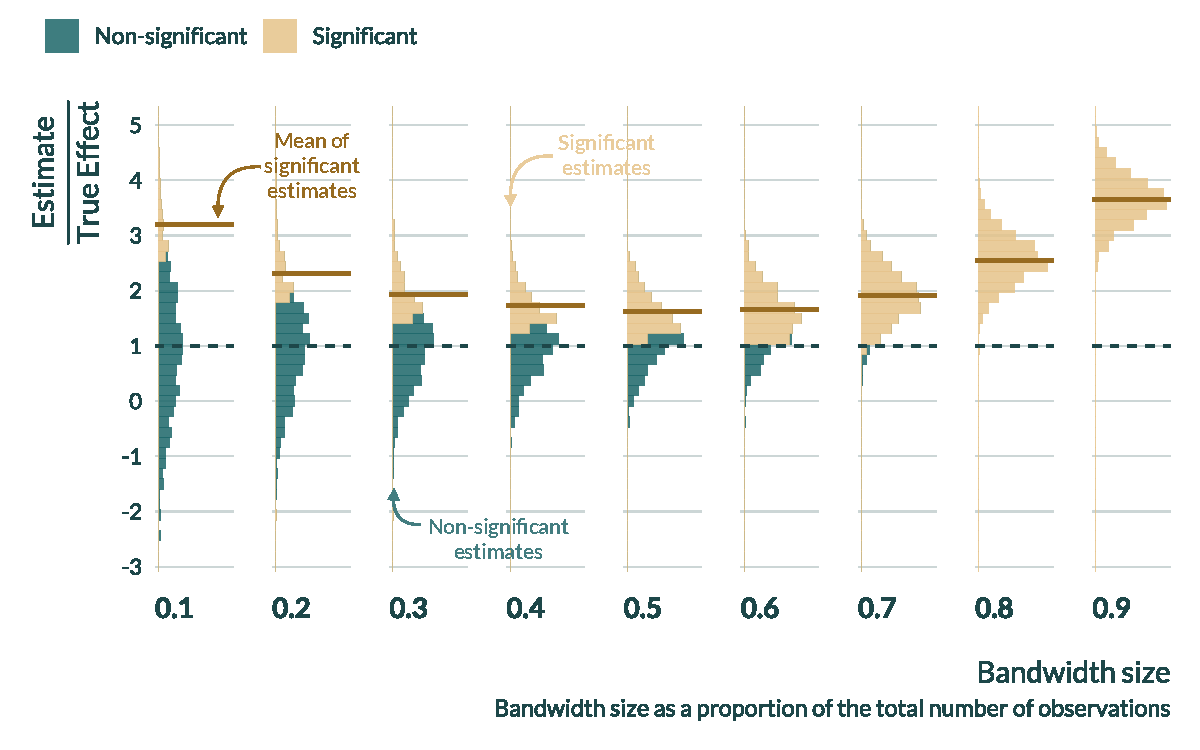
\includegraphics[width=0.8\linewidth]{images/main_graph_RDD_paper_annotated.pdf}
		      			\caption*{\footnotesize \textit{Notes}: 1000 simulations. Significativity level: 5\%, N = 60,000. The brown lines represent the average of significant estimates. The bandwidth size is expressed as the proportion of the total number of observations in the entire sample. Details on the simulation are available at this \href{https://vincentbagilet.github.io/causal_exaggeration/RDD.html}{link}.}
				\end{center}
				\vspace{-1cm}
			\end{figure} 
		

		
		
%%%%%%%%%%      SIM    Controls        %%%%%%%%%%%%%%%
		
		 \subsection{Fixed Effects and Controlling for Confounders}\label{sim_ctrl}
		
     			\paragraph{Intuition.} To identify a causal effect and avoid the risk of confounding, an ``ideal'' approach would be to partial these confounders out by directly controlling for them. % by including additional variables in the regression model to eliminate endogenous variation. In the ideal case, we would control for the omitted variable and for this only. 
			However, as discussed in the introduction and section \ref{maths}, controlling for an additional variable may increase the variance of the estimator if it absorbs more variation in the explanatory variable of interest than in the outcome variable.
			% ($y$). Controlling for a variable ($w$) is equivalent to partialling out this variable from both $x$ and $y$. Since the variance of the OLS estimator is given by the ratio of the variance of the residuals $\sigma_{y^{\perp x, w}}^2$ over $n$ times the variance of the explanatory variable after partialling out $w$ ($\sigma_{x^{\perp w}}^2$), if controlling absorbs more of the variance in $x$ than in $y$, it will increase the variance of the resulting estimator and create exaggeration. 
			The same reasoning applies to a cornerstone causal identification approach: Fixed Effects (FEs). If including FEs partials out more of the variation in $x$ than in $y$, it will increase the variance of the estimator and can lead to exaggeration. 
			
			\paragraph{Case-study and simulation procedure.} To highlight this trade-off, I consider the case of studies on the impact of temperature on worker productivity. A typical approach in this literature consists in estimating the link between different temperature bins and productivity, focusing in particular on high temperature bins \citep[for a review of the literature]{lai_effects_2023}. Usual approaches to explore this question typically rely on High Dimensional Fixed Effects models, including time and location fixed effects to adjust for invariant characteristics such as seasonal demand or location differences. For readability, in my simulations I only consider time fixed effects and abstract from location ones. I assume that the true data generating process for temperature at time $t$ in period $\tau$ is $Temp_{t\tau} = \mu_{Temp} +  \gamma\lambda_{\tau} + \epsilon_{t}$ where $\mu_{Temp}$ is an intercept representing the average temperature and $\lambda_{\tau}$ are period fixed-effects with mean 0 and variance 1, such that their variance can be modified \textit{via} $\gamma$. This particular structure of fixed effects allows controlling for the intensity of the fixed effects via the parameter $\gamma$, determining the proportion of the variation in temperature that comes from period-to-period (month) variations in average temperature. The productivity of worker $i$ is defined as $Prod_{it\tau} = \beta_0 + \eta_i + \delta\lambda_{\tau} + \beta_1 \cdot \mathbbm{1}\{Temp_{t\tau} \in (T_L,T_H ] \} + u_{it}$ where $\eta_i$ are individual fixed effects and $(T_L,T_H ]$ the temperature bin of interest. The effects for other bins are  not simulated and set to zero. For the omitted variable bias to remain constant when $\gamma$ varies, I fix $\kappa = \gamma\delta$. I also adjust for the variances of $\epsilon$ and $\eta$ to keep the variance of $x$ and $y$ constant.
			
			I calibrate my simulations to replicate the distribution of the variables and interactions between variables from a typical study from the literature of interest \citep[among others]{stevens_temperature_2017,somanathan_impact_2021,lai_effects_2023,lopalo_temperature_2023}. A more detailed description of calibration and modeling choices is available on the \href{https://vincentbagilet.github.io/causal_exaggeration/FE.html#calibration-and-baseline-parameters-values}{project's website}. For each value of $\gamma$, or equivalently each proportion of the variation in temperature that is period-specific considered, I generate 1000 datasets with 49,000 observations and estimate two models, one including and the other omitting period fixed effects. The SNRs obtained are in line with many of those observed in the literature.
				
			%IMPORTANTLY, ADDING FIXED-EFFECTS OFTEN MODIFIES THE ESTIMAND, MAKING FAKE-DATA SIMULATIONS EVEN MORE CRUCIAL IN THIS SETTING. (CAUSE IN REAL SETTING CANNOT KNOW THE TRUE EFFECT)
        
       			 \begin{figure}[!h] 
				\begin{center}
					\caption{Evolution of the Bias with the Proportion of the Variance in X explained by the Fixed Effects, for Statistically Significant Estimates.}
					\label{graph_fe}
					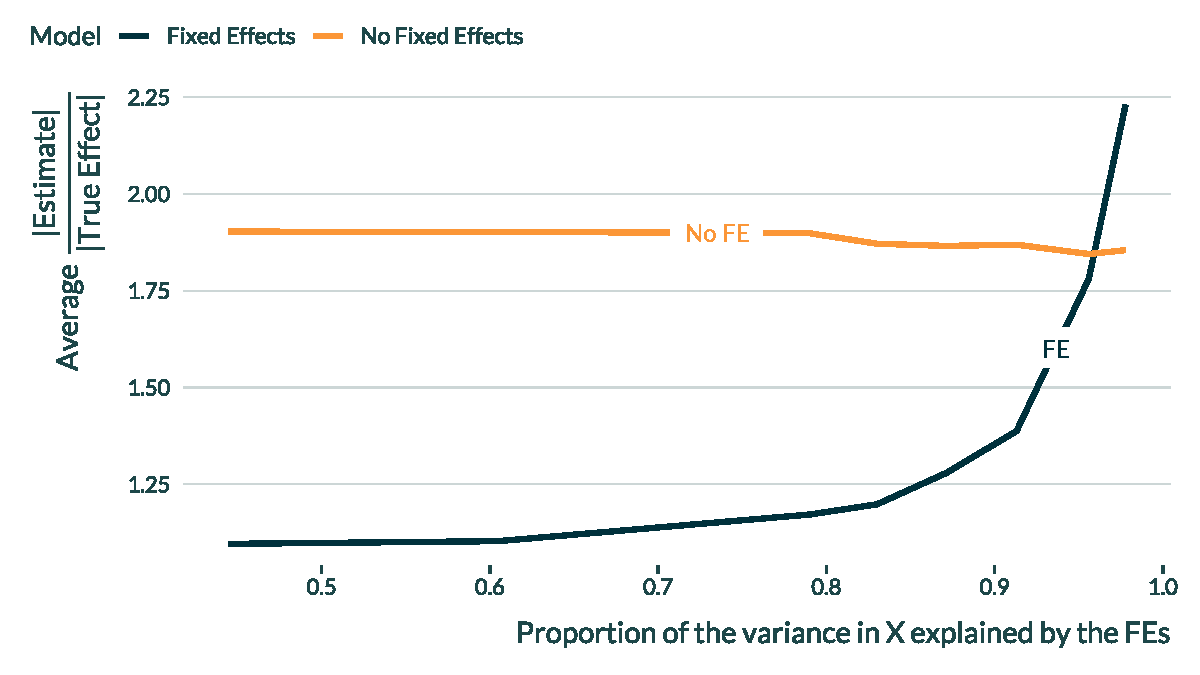
\includegraphics[width=0.8\linewidth]{images/main_graph_fe_paper_annotated.pdf}
		      			\caption*{\footnotesize \textit{Notes}: The blue line indicates the average bias for estimates from the model including FEs that are statistically significant at the 5\%. The orange line represents the bias of statistically significant estimates from the model without the fixed effects. In this simulation, N = 50,000. Details on the simulation and calibration are available at this \href{https://vincentbagilet.github.io/causal_exaggeration/FE.html}{link}.}
				\end{center}
				\vspace{-1cm}
			\end{figure} 
			
			\paragraph{Results.}  Figure \ref{graph_fe} displays the results of these simulations. When the (period) fixed effects explain a large part of the variation in $x$ (temperature), the estimator is imprecise and leads to exaggeration, to the point that it becomes larger than the OVB simulated.
			While this phenomenon arises when fixed effects explain a relatively important share of the variance in temperature, it remains non-negligible for month-to-month variations in temperature routinely observed in actual situations. In addition, this setting presents large effect sizes and relatively large samples; other settings with smaller effect and sample sizes likely exhibit substantial exaggeration for smaller shares of variation captured by fixed effects. The inclusion of additional fixed effects might also further increase exaggeration.

%%%%%%%%%%      SIM    IV        %%%%%%%%%%%%%%%
		
        		\subsection{Instrumental Variables Strategy}\label{sim_IV}
            
                		\paragraph{Intuition.} 
        			Instrumental variables strategies overcome the issue of unobserved confounding by only considering the exogenous variation in the treatment, \textit{i.e.} the variation that is explained by the instrument. Even when this exogenous fraction of the variation is limited, the instrument can successfully eliminate confounding on average. However, in such cases, the IV estimator will be imprecise and statistical power low. In the case of the IV, the confounding-exaggeration trade-off is mediated by the strength of the instrument considered. The weaker the instrument, the more inflated statistically significant estimates will be.
        		
        			\paragraph{Case-study and simulation procedure.} 
        			To illustrate this trade-off and its drivers, I consider the example of the impact of voter turnout on election results. To avoid the threat of confounding in this setting, existing studies take advantage of exogenous factors such as rainfall that affect voter turnout.\footnote{I abstract from potential exclusion restriction violations of this instrument and simulate it as exogenous.} I reproduce such setting and assume that the true data generating process for the republican vote share is such that  in location $i$, $Share_{i} = \beta_{0} + \beta_{1} Turnout_{i} + \delta w_{i} + u_{i}$, where $w$ is an unobserved variable and $u \sim \mathcal{N}(0, \sigma_{u}^{2})$ some random noise. The causal parameter of interest is $\beta_{1}$. In addition, turnout is affected by the amount of rain: $Turnout_{i} = \pi_{0} + \pi_{1} Rain_{i} + \gamma w_{i} + e_{i}$, where $Rain_{i}$ is the amount of rain in location $i$ on the day of the election 
			%\footnote{In the DiD event study simulations that reproduce this setting, $Rain_{i}$ is a dummy for whether it rained or not on the day of the election in location $i$.} 
			and $e$ some random noise drawn form $\mathcal{N}(0, \sigma_{e}^{2})$. I refer to $\pi_{1}$ as the strength of the instrumental variable. 
        			
        			To make the simulations realistic, I calibrate them on existing studies. I derive sample size, distribution parameters and effect sizes from a set of studies using similar variables \citep{gomez_republicans_2007, fujiwara_habit_2016, cooperman_randomization_2017}. Details on the calibration choices are available on the \href{https://vincentbagilet.github.io/causal_exaggeration/IV.html#calibration-and-baseline-parameters-values}{project's website}. For each value of IV strength considered, I create 1000 datasets of 30,000 observations. I run both a naive OLS and a 2SLS model to estimate the impact of voter turnout on republican vote share. SNR obtained are aligned with SNR observed in this literature.
        			
        		
                    		 \begin{figure}[!h] 
                    			\begin{center}
                    				\caption{Evolution of the Bias of Statistically Significant Estimates Against Strength of the Instrument in the IV Case.}
                    				\label{graph_IV}
                    				\includegraphics[width=0.8\linewidth]{images/main_graph_IV_paper_annotated.pdf}
                                    \caption*{\footnotesize \textit{Notes}: The blue line indicates the average bias for IV estimates that are statistically significant at the 5\%. The orange line represents the bias of statistically significant OLS estimates at the 5\% level. The strength of the instrumental variable is expressed as the value of the linear parameter linking rainfall to turnout. In these simulations, N = 30,000. Details on the simulation are available at this \href{https://vincentbagilet.github.io/causal_exaggeration/IV.html}{link}.}
                                    \end{center}
				\vspace{-1cm}
                    		\end{figure} 
		
		\paragraph{Results.} 
			Figure \ref{graph_IV} displays, for different IV strengths, the average of statistically significant estimates scaled by the true effect size for both the IV and the naive regression model. When the instrument is strong, the IV will recover the true effect, contrarily to the naive regression model. Yet, when the IV strength decreases, the exaggeration of statistically significant estimates skyrockets. Even if the intensity of the omitted variable bias is large, for limited IV strengths, the exaggeration ratio can become larger than the omitted variable bias. When the only available instrument is weak, using the naive regression model would, on average, produce statistically significant estimates that are closer to the true effect size than the IV. Of interest for applied research, a large $F$-statistic does not necessarily attenuate this problem. This result complements limitations around the use of first-stage $F$-statistics with non-iid errors \citep{young_consistency_2022,lalHow2024}.
			%For the parameter values considered here, this phenomenon arises even in cases for which the $F$-statistic is substantially larger than the usually recommended threshold of 10, as illustrated in the \href{https://vincentbagilet.github.io/causal_exaggeration/IV.html#f-statistic-analysis}{online supplementary materials}. 
		
% I start with the RDD and matching cases because in these settings the researcher has a hand on the parameter driving power: the bandwidth size and the stringency of the matching mechanism.



%%%%%%%%%%      SIM    EVENT        %%%%%%%%%%%%%%%

		\subsection{Exogenous shocks}\label{sim_shocks}
    
        			\paragraph{Intuition.}  Taking advantage of exogenous variation in the treatment status caused by exogenous shocks or events can also enable avoiding confounding. In many settings, while the number of observations may be large, the number of events, their duration or the proportion of individuals affected might be limited. As a consequence, the number of (un)treated observations can be small and the variation available to identify the treatment limited. As extensively discussed in the randomized controlled trial literature, statistical power is maximized when the proportion of treated observations is equal to the proportion of untreated ones and drops when one of these proportions gets close to 0. In studies using discrete exogenous shocks, a confounding-exaggeration trade-off is thus mediated by the number of treated observations. %This issue does not only concern DiD event studies but is particularly salient in this case. 
			
			\paragraph{Case-study and simulation procedure.} %To illustrate this trade-off, I reproduce the analysis described for instrumental variable strategies described in section \ref{sim_IV} but considering that $Rain$ is a dummy equals to one if it rained on the day of the election.
			To illustrate this trade-off, I simulate a study of the impact of air pollution reduction on newborn weight of babies. To avoid confounding, one can exploit exogenous shocks to air pollution such as plant closures, creation of a low emission zone or of an urban toll \citep{currie_environmental_2015, lavaine_energy_2017}. I simulate a typical analysis, at the zip code and monthly levels and focus on the example of toxic plant closures. I consider that the average birth weight in zip code $z$ at time period $t$, $bw_{zt}$, depends on a zip code fixed effect $\zeta_z$, a time fixed effect $\tau_t$, and the treatment status $T_{zt}$, equal to one if a plant is closed in this period and 0 otherwise. The average birth weight in zip code $z$ at time $t$ is defined as follows: $bw_{zt} = \beta_0 + \beta_1 T_{zt} + \zeta_z + \tau_t + u_{zt}$. To further simplify the identification of the effect, I assume a non-staggered treatment allocation and constant and homogenous effects. I only vary the proportion of zip codes affected by toxic plant closings, keeping the length of the closures fixed.

       I derive parameters values from studies from the literature \citep{currie_environmental_2015, lavaine_energy_2017}. The simulations mimic the design of such studies, considering a similar number of observations (150,000), distributions of variables, treatment allocation procedure and treatment effect sizes. I generate datasets with an increasing number of treated observations, varying the proportion of treated units and estimate the correct two-way fixed effects model. The simulation procedure is described in details on the \href{https://vincentbagilet.github.io/causal_exaggeration/shocks.html}{project's website}.
        
			\paragraph{Results.} Figure \ref{graph_shocks} displays the results of these simulations. As expected, exaggeration is larger for a smaller number of treated observations, keeping every thing else constant. Even though the actual sample size is extremely large in this example, if the number of treated observations is small, as it can be the case in this literature, exaggeration can be substantial. A very large number of observations does not necessarily shield us from exaggeration. 

			\begin{figure}[!h] 
                    			\begin{center}
                    				\caption{Evolution of Bias With the Number of Treated Observations, for Statistically Significant Estimates, in the Exogenous Shocks Case}
                    				\label{graph_shocks}
                    				\includegraphics[width=0.8\linewidth]{images/main_graph_DID_paper.pdf}
                                    \caption*{\footnotesize \textit{Notes}: Significance level: 5\%. In this simulation, N = 150,000. 1000 iterations for each number of treated observations considered. Details on the simulation are available at this \href{https://vincentbagilet.github.io/causal_exaggeration/shocks.html}{link}.}
                                    \end{center}
				\vspace{-1cm}
                    		\end{figure} 
		
		
%-----------------------------------------------------------------------------

% PRACTICAL RECOMMENDATIONS

%-----------------------------------------------------------------------------

	\section{Navigating the trade-off} \label{discussion}

		% HOOK OF THE SECTION
 		In the previous sections, I showed using causal identification strategies induces a trade-off between avoiding confounding and exaggerating true effects. How can we, as applied researchers using observational data, arbitrate it? Since key pieces of information such as the true effect and the effect of omitted variables are inherently unknown, we cannot directly compute the biases caused by confounders and exaggeration. In this section, I examine how we can, however, get a sense of threats from both sides of the trade-off and probe its main driver, the variation used for identification. I then discuss how changing attitudes towards statistical significance and replicating studies could limit the exaggeration issue.
	
	%Even though it does not produce uninflated estimates, reporting power calculations enables to evaluate the risk of exaggeration for a study. In this section, we present a workflow to evaluate and report the power of a study before and after its implementation. 
	
		\subsection{Gauging omitted variable bias}
	
			%"MEASURING" OVB
			On one side of the trade-off lies the widely discussed bias caused by confounders. Although it is in essence impossible to measure, tools such as sensitivity analyses are available to gauge its magnitude \citep{rosenbaum_observational_2002, middleton_bias_2016, oster_unobservable_2019, cinelli_making_2020}. For instance, the method developed in \cite{cinelli_making_2020} enables assessing how strong confounders would have to be to change the estimate of the treatment effect beyond a given level we are interested in. It offers bounds for the strength of the association between the treatment and potential omitted variables by weighting it against the measured association between the treatment and observed covariates. A typical conclusion from such an analysis would be: ``omitted variables would have to explain as much residual variance of the outcome and the treatment as the observed covariate $x$ (age for instance) to bring down the estimate to a value of $\beta_{l}$''. The authors also implement graphical tools to facilitate this comparison. I suggest using quantitative bias analyses to assess how restrictive a causal approach must be to limit unobserved confounding to acceptable levels. Extremely strict controls and fixed effects may leave little scope for confounders but can generate substantial exaggeration. In such situations, the potential influence of confounders should be weighed carefully: given the risks of exaggeration---and concerns about representativity---causal estimates should not be treated as definitive benchmarks for assessing naive estimates, nor should a discrepancy between the two be taken as sufficient evidence that the naive estimate is incorrect.
			
		\subsection{Evaluating risks of low power and exaggeration}

			On the other side of the trade-off lies the exaggeration emerging when statistical power is low. As OVB, exaggeration and statistical power are in essence impossible to measure as their computation depends on the true effect which is always unknown. Yet, power calculations can help assess them by making hypothesizes on the magnitude of the true effect. In randomized controlled trials, such computations are not only an established practice but a requirement \citep{duflo_using_2007, mcconnellGoingSimpleSample2015, athey_econometrics_2016}. They are, however, rarely reported in non-experimental studies. %This can be understandable if power calculations are perceived only as a way to measure a design's ability to detect an effect. 
			Yet, taking publication bias and the threat of exaggeration into account highlights the necessity of running power calculations in non-experimental studies as well. A low power or a relatively large variance not only makes it more difficult to detect an effect or to draw clear conclusions about its magnitude when detected but it can also create a bias. To avoid this bias, I advocate to make power more central to non-experimental analyses. Currently, in causal inference textbooks, very few pages are devoted to statistical power in non-experimental studies \citep{angrist_mostly_2009, angrist_mastering_2014, imbens_causal_2015, cunningham_causal_2021}. To the best of my knowledge, only two textbooks discuss the matter in depth \citep{shadish_experimental_2002, huntington-klein_effect_2021}. Results from power and exaggeration calculations would not only be highly informative but would also be very easy to report in the robustness section of articles. 
			
			\subsubsection{Prospective power calculations}
						
				To evaluate the statistical power of a study, the risk of exaggeration and identifying the factors driving it, one can simulate the design of the study before implementing it \citep{hill_bayesian_2011, gelman_regression_2020, black_simulated_2022}. %add 
				Simulating a data generating process from scratch requires thinking about the distribution of the variables, about their relationships and can also help underline the variation used for identification. %External information found in previous studies can help guide the simulation process to make it more realistic. 
			 I implemented such Monte Carlo simulations in \Cref{simulations}. The replication material and \verb?R? code I provide can be used as an example to implement simulations for most causal identification strategies, based on data generated from scratch. In situations where the relationships among covariates are too complex to emulate, one can also start from an existing dataset and add a fake and known treatment effect to the data. I implemented such real-data simulations in a companion paper and describe their implementation in its \href{https://vincentbagilet.github.io/inference_pollution/}{replication material} \citep{bagilet_accurate_2023}. 
			 
			 %When simulations indicate that statistical power is low, additional data could be collected or the statistical model could be improved to increase precision. In any case, it should not stop the research project from carrying out. Simulation results rest on the way the data generation process was modeled, and it can be difficult to gauge the amount of noise present in data before actually analyzing them. The two main benefits of a prospective simulation procedure are that it allows us to consider factors that may affect the statistical power of our study and to avoid drawing misleading conclusions based solely on statistically significant estimates when statistical power is low.
				
			\subsubsection{Retrospective power calculations}\label{retro_calc}
			
				Running post-analysis power calculations can also help getting a sense of the statistical power associated with a research design, as seen in section \ref{lit_review}. Such \textit{retrospective} calculations allow evaluating whether the design of the study would produce accurate and uninflated statistically significant estimates if the true effect was in fact smaller than the observed estimate \citep{gelman_beyond_2014, ioannidis_power_2017, stommesReliability2023}. 
				
				%can take this out if want to make the paper shorter
				I illustrate how a retrospective analysis works by taking the example of \cite{card_using_1993} on the relationship between human capital and income. The IV strategy in this paper finds that an additional year of education, instrumented by the distance of growing up near a four-year college, causes a 13.2\% average increase in wage, with an associated standard error of 5.5\%. Is there a risk of exaggeration with this design? Since, as noted by the author himself, the estimate is very imprecise we could expect so. Imagine the existing literature suggests that such effects are likely to be close to a 10\% increase in wage. We may wonder if the design in \cite{card_using_1993} would allow detecting such an effect. We can thus easily compute the statistical power and exaggeration of \citeauthor{card_using_1993}'s design under the hypothesis of a true effect size of 10\%.\footnote{\cite{timm_retrodesign_2019} and \cite{linden_retrodesign_2019} offer \texttt{R} and \texttt{Stata} packages that enable easily running these calculations through an extremely short command: \texttt{retrodesign(10, 5.5)}. As discussed previously, the exaggeration is computed by drawing a large number of times from a normal distribution centred on the hypothetical effect size of 10\% and with a standard deviation equal to the standard error of the estimate found in the study (here 5.5\%) and by then computing the average of the absolute value of the draws that are 1.96 standard errors away from 0.} The average statistically significant estimate at the 5\% level would be roughly of 15\%, therefore overestimating the true effect by a factor of 1.5. Statistical power would only be 44\%. Conditional on a 10\% true effect size being a reasonable assumption, this design would be under-powered and exaggeration substantial. 
			
				The usefulness of any retrospective power analysis lies on the assumption made regarding the true effect size. To identify a range of plausible effect sizes one can rely on results from meta-analyses or from existing studies that have a credible design (\textit{e.g.}, a large randomized controlled trial). When such meta-analyses are available, one can use Bayesian shrinkage to adjust statistically significant estimates in light of the distribution of estimates obtained in prior studies \citep{zwet_proposal_2021, zwet_significance_2021, zwet_statistical_2021}. When such information is not available, power calculations can be ran for a range of smaller but credible effect sizes that can be for instance derived from theoretical findings. It is also possible to evaluate whether the design of our study would be able to detect smaller effects than the point estimate obtained, while keeping in mind that there might be shortcomings to this approach as the obtained estimate or previously published ones may themselves be exaggerated \citep{gelman_beyond_2014}.
				
		%\subsection{Driver of the trade-off}
		
			%We have seen that the variation used for identification was the main driver of the confounding-exaggeration trade-off. This variation determines the variance of the estimator and thus the amount of exaggeration. In this section, I first discuss the impact of estimator variance and how exaggeration leads to reinterpret the well-known bias/variance trade-off. I then propose to use a tool that enables visualizing where the variation used for identification comes from.
		
			\subsubsection{Precision matters even after obtaining a significant estimate}
			
				In non-experimental studies, estimator variance often plays a critical role because a large variance may prevent rejecting the null hypothesis when it is false. As a result, variance is typically a central concern until a statistically significant estimate is obtained. However, exaggeration highlights that variance remains important for the reliability of the point estimate---and for reasons beyond mere uncertainty---even after statistical significance has been achieved.
			
				 Obtaining a statistically significant estimate from an imprecise estimator should not necessarily be interpreted as a sign of ``success'' in getting significance despite a wide confidence interval. Rather, it may signal that this estimate liens in the tails of the distribution and thus inaccurately represents the true effect. %Conditional on having obtained a statistically significant estimate, a limited precision can hide a bias: exaggeration. 
				This observation reframes the conventional bias-variance trade-off as a bias-bias trade-off: a larger variance can lead to a larger bias, even in (conditional) expectation. This paper therefore calls for careful attention to the implications of design and modeling choices on estimator variance, even when large variance has not prevented statistical significance.
			
		\subsection{Identifying the identifying variation}
		
			\subsubsection{A metric of identifying observations}
				
				%It might then seem compelling to define this effective sample by proposing a weight value under which the associated observation does not actually contribute to  identification. Yet, considering the specificity of each analysis and that exaggeration depends on several factors, including the true effect size, I instead suggest to visualize the individual weights.\footnote{In future developments of this project, I will however develop a measure of this effective sample size. I may also need to modify the weights formula in order to account for the variation in $y$ that is absorbed when controlling.}  It allows getting a sense of where the variation comes from and which are the observations that actually contribute to the estimation. Since applied economic analyses often rely on panel data, I propose to use a heatmap as a base for visualization, with time on the \textit{x}-axis and individuals on the \textit{y}-axis. If the data is geographical, one can directly plot the weights on a map.%cross sectional, the same heatmap can be computed with individuals on the \textit{x}-axis and a length-one segment on the \textit{y}-axis.\\
				
				%\textit{I still need to develop an example. The one I have, based on \cite{deschenes_economic_2007} is actually not a good example because their effect is a composite of various effects. I need to identify another paper. In addition, I need to think again about my metric because it needs to represent the ratio of the residual variance (after partialling out fixed effects) of $y$ over that of $x$.}
				
				The approaches outlined above for assessing exaggeration and confoundings are built on assumptions regarding the true effect size. To circumvents these assumptions, one can instead directly focus on the driver of the bias-variance trade-off: the variation used for identification. When the identifying variation is too limited, statistical power is low and exaggeration is large. Pinpointing the specific variation on which estimation relies can provide a direct way to gauge the risk of exaggeration. This section introduces tools to identify that variation.
			
				To identify the identifying variation in an applied study, one usually begins with a thought exercise: where does the variation leveraged for identification come from? This reflection is integral to the implementation of any applied economics study. While it is typically undertaken primarily for identification and internal validity purposes, this paper also highlights its importance for exaggeration reasons, \textit{i.e.} after a significant estimate has been obtained. Although this exercise may be straightforward in simple cases---such as one-way fixed effects---it becomes more challenging in complex designs involving multiple or interacting fixed effects, especially for readers less familiar with the setting.
			
				Given this difficulty of intuitively identifying the source of variation in complex models, it can be useful to develop measures that quantify the contribution of each observation or group of observations to the estimation of the treatment effect. A range of existing tools from the statistics literature, such as leverage and Cook’s distance, measure the influence of individual observations on regression parameters. These measures, however, assess influence on the \textit{entire} parameter vector and are not directly suited for applied economics where interest is typically confined to a single parameter: the coefficient of the treatment variable. To get to a more suited measure, I propose to first apply the Frisch-Waugh-Lovell theorem and then compute leverage for the regression of the residualized outcome on the residualized treatment. The residuals are obtained from regressions on the full set of controls, including fixed effects and other identification-related controls such as control functions. This produces observation-specific weights describing the extent to which each observation contributes to the estimation of the treatment effect. 
			
				These weights are equivalent---up to a normalization to one---to the multiple regression weights introduced in \cite{aronow_does_2016} and previously discussed in \cite{angrist_mostly_2009}. %, section 3.3.1.
				The estimate of the treatment coefficient in a simple linear regression can be interpreted as a weighted average of individual treatment effects. The weight $\omega_{i}$ of individual $i$ is the squared difference between its treatment status $T_{i}$ and the value of this treatment status as predicted by the other covariates $X$: $\omega_{i} = (T_{i} - \mathbb{E}[T_{i} | X_{i}])^{2}$. %AAADDD prooof to the appendix 
				%ADDDD THAT THESE WEIGHTS KICK IN AS SOON AS THE INDEPENDENCE ASSUMPTION DOES NOT HOLD (AND THAT NEED SOME SORT OF CIA)
				At the group level, these weights connect to well-established insights, particularly in the widely used case of fixed effects. A group’s weight, \textit{ie} the sum of the individual weights within that group, corresponds to the within-group variance of the conditional treatment status. Since including fixed effects changes the type of variation used for identification from pooled to within-group variation, groups with little within variation in treatment status only marginally contribute to identification. 
				These weights also have crucial implications at the observation level: individual observations whose treatment status is largely explained by covariates contribute little, if at all, to estimation. Variation in the explanatory variable of interest is absorbed by the controls. In that sense, the weights not only highlight the role of groups but also the uneven contribution of individual observations within them. More broadly, in settings without a natural grouping structure, observation-level weights help assess how much each unit actually contributes to identification. 
				\cite{aronow_does_2016} uses these weights to argue that, when treatment effects are heterogeneous, some observations may be disproportionately represented in the estimated average effect, raising concerns about external validity. Even in the absence of heterogeneity, however, relying on observations whose treatment status is well explained by covariates can yield a very small \textit{effective} sample size and, in turn, exaggeration. Whereas \cite{aronow_does_2016} emphasizes the representativity of the effective sample for external validity reasons, the present paper focuses on its size, for fear of exaggeration.
			
			\subsubsection{A tool to identify the identifying variation}
			
				Although the computation of these weights is relatively straightforward, it involves several steps, and their subsequent analysis and comparison are more challenging. To facilitate this process, I develop the \href{https://vincentbagilet.github.io/ididvar/}{\verb?ididvar? package} for \verb?R?.\footnote{This package can be extended to accommodate more specific settings. Readers are encouraged to suggest improvements through \href{https://github.com/vincentbagilet/ididvar}{GitHub issues or pull requests}.} The package provides a unified tool to compute identifying-variation weights and related contribution metrics, along with a series of visualization tools. 
				 By lowering the cost of identifying which observations drive estimation, the package aims helping assess potential risks of exaggeration when identifying variation is limited. Unlike power calculations, these metrics can be computed without assumptions about the true effect size.
			
				Most functions are high-level and easy to use, requiring only the regression output and the variable of interest. A first set of functions computes and visualizes weights, including their distribution across space, groups, or time. This enables users to detect low-weight observations or clusters that contribute little to identification. Because the distribution of weights is often heterogenous, building meaningful visualization can be challenging. To address this, I propose a discretized and logged scale that compares each weight to the average weight, $1/n$, where $n$ is the number of observations or groups. This representation clarifies variation and ensures comparability across specifications and studies.
				
				To illustrate the package’s features, I consider a simple example using a country-level panel \citep[restricted to Africa and Europe for clarity]{bryan_jennybc_2017} and estimate the within-country relationship between GDP per capita and life expectancy:  $\log(PerCapitaGDP_{ct}) = \alpha_c + \beta LifeExp_{ct} + u_{ct}$. Figure \ref{graph_ididvar} presents visualizations produced by the package. Panel A displays the identifying-variation weights for each observation,\footnote{This graph is essentially generated in one line of code:\\$\verb?idid\_viz\_weights(reg, ''l\_gdpPercap'',  year, country)?$ where $\verb?reg?$ is the output of the regression of interest, $\verb?l\_gdpPercap?$ the variable of interest and $\verb?var\_x?$ and $\verb?var\_y?$ specify the variables to be displayed n the $x$ and $y$-axes respectively} while Panel B shows their cumulative distribution. The distribution is highly heterogeneous: many observations contribute little to identification, particularly those from mid-periods and European countries.
				
				Weights alone, however, do not indicate which observations actually contribute to identification. A second set of functions identifies the \textit{effective sample}: the smallest subset of observations that cannot be removed without altering the point estimate or standard error of the parameter of interest by more than a chosen margin, e.g., 5\%.  The procedure iteratively re-estimates the model, removing low-weight observations following an approach similar to influence-function methods. Reporting the effective sample size helps interpret results in light of the sample that actually drives identification, much as one would interpret the nominal sample size. It does not, however, imply that these observations should be excluded from the main estimation.
				
				\begin{landscape}
				\begin{figure}[ht]
					\caption{Illustration of the types of analyses ididvar allows}
					\label{graph_ididvar}
					\includegraphics[height=0.9\textheight]{images/ididvar.pdf}
					\caption*{\footnotesize \textit{Notes}: Details on the computation are available at this \href{https://vincentbagilet.github.io/causal_exaggeration/ididvar.html}{link}.}
				\end{figure}
				\end{landscape}
				
				In the illustrative example, Panel C of Figure \ref{graph_ididvar} shows how point estimates and standard errors evolve as low-weight observations are sequentially dropped. 70\% of the nominal sample can be dropped without affecting estimates and standard errors that differ by more than 5\%. The effective sample is thus about three times smaller than the nominal sample.  Results should be interpreted accordingly. Panels D and E characterize this effective sample: many observations from Africa and mid-periods do not contribute to identification, implying that the effective sample is not representative of the full dataset.
				
				The package is flexible and can be applied to a wide range of identification strategies and estimation methods. It enables users to compare specifications and explore how the inclusion of different sets of fixed effects or controls affects the effective sample. More broadly, by making the structure and amount of identifying variation explicit, the package provides a concrete way to assess where a study lies along the confounding-exaggeration trade-off. In doing so, it aims to help users evaluate whether the credibility gained from additional controls comes at the cost of a loss of identifying variation and statistical power.
			
				
		% GENERAL RECOMMENDATIONS
		\subsection{Attitude Towards Statistical Significance and Replication}
	
			Exaggeration only arises in the presence of publication bias. As shown in the simulations, if estimates were not filtered by their statistical significance nor any other characteristics, even under-powered studies would on average recover the true effect, as long as the estimator is unbiased. The exaggeration issue could therefore be addressed by tackling publication bias.\footnote{Note that even if this publication bias is often understood as selection of statistical significance, it can also extend to any situation in which a certain type of results, large or surprising for instance, are favored. The present paper focuses on the former type of selection owing to its primacy and the fact that its existence and the mechanisms causing it are well-documented.}
		
			To identify broader pathways to eliminate this filtering of significant results, it is first helpful to discuss the processes that lead to statistically significant results when power and thus the probability of obtaining a significant estimate is low. In such situations, they can be obtained either by ``chance'' or as an outcome of the garden of forking paths \citep{simmons_false-positive_2011, gelman_garden_2013, kasy_forking_2021}. Decision forks appear at various stages along the path of research, for instance in data preparation, regarding the inclusion of a given control variable in the model or observation in the sample or later, regarding whether to carry on with a research that yields non-significant results. Due to the structural flaw that favors significance, the path followed may be more likely to lead to a statistically significant result. These choices are most often not the result of bad researcher practices but instead a product of a structure that portrays significant results as an end goal of research. 
		
			The issue being structural, system level changes in scientific practices could also alleviate exaggeration and the trade-off described in this paper. First, many researchers advocate abandoning statistical significance as a measure of a study's quality \citep{mcshane_abandon_2019}. To be effective, this change should be paired with an effort to replicate studies \citep{christensen_transparency_2018}. Replications, even of low powered studies, would eventually enable building the actual distribution of the causal estimand of interest. Meta-analyzes would then reduce the uncertainty around the true value of the causal estimand by pooling estimates \citep{hernan_causal_2022}. Finally, the inflation of statistically significant estimates could be limited by interpreting confidence intervals and not point estimates and thus considering these intervals as compatibility intervals \citep{shadish_experimental_2002, amrhein_inferential_2019, romer_praise_2020}. The width of such intervals gives a range of effect sizes compatible with the data. These intervals will be wide in under-powered studies signalling that point estimates should not be taken at face value, even if statistically significant.

%-----------------------------------------------------------------------------

% CONCLUSION

%-----------------------------------------------------------------------------

\section{Conclusion} \label{conclusion}

	The economic literature suffers from an extensive lack of statistical power \citep{ioannidis_power_2017} and strongly favors statistically significant findings \citep[for instance]{rosenthal_file_1979, andrews_identification_2019, abadie_statistical_2020, brodeur_methods_2020}. In such situations, significant estimates from underpowered studies always exaggerate true effect sizes, even when the estimators are ``unbiased'' in the usual sense of $\mathbb{E}[\hat{\beta}] = \beta$ \citep{gelmanType2000, ioannidis_why_2008, gelman_beyond_2014}. It is therefore not surprising that many estimates published in economics have been found to be considerably exaggerated \citep{ioannidis_power_2017}, despite the extensive use of convincing causal inference methods. Yet, the determinants of these exaggeration and power problems have remained largely understudied. I argue that exaggeration is exacerbated by the foundational component of causal inference: the fact that it only leverages subsets of the variation for identification. Although causal methods enable avoiding confounding, they also reduce statistical power and thus increase the risk of exaggeration. The same aspect that makes these methods credible can create another type of bias. Systematically reporting statistical power and examining the variation actually used for identification could help avoid falling into this exaggeration trap.

%-----------------------------------------------------------------------------

% NEXT STEPS

%%-----------------------------------------------------------------------------
%
%\section{Next steps} \label{next_steps}
%
%	Here is an ordered list of the next tasks I plan to do. I would love to get feedback on both the content and the order of this list. Are there more urgent points than others? Are there other things I need to add to this list?\\
%
%	\textit{For each task, I write down what section of the paper it pertains to (S = Simulations, M = Maths, R = Recommendations, W = Writing). Question marks mean that I am not certain that this task is necessary.}\\
%
%	\begin{enumerate}
%		\item (S) Verify the SNR in my simulations: are they similar to those in the published papers?
%		\item (S) Add more visualizations
%		\item (S) Calibrate simulations for FEs/controls
%		\item (W) Add an actual example for controls: in a real data set, compare exaggeration when a given variable is used as a control or not + try to find existing papers for which adding more and more FEs increases variance
%		\item (W) Expand the description of the simulations in the body of the paper (and move matching and exogenous shocks to the appendix) + add the simulation codes (my RMarkdown files) to the appendix
%		\item (W) Add a literature review describing the extent of exaggeration in a literature (either acute health effects of air pollution, \textit{i.e.}, directly reinjecting my other paper or adding something different  based on Leo's work on interventions aimed at reducing household energy consumption or on behavioral interventions to promote household action on climate change)
%		\item (R) Add discussion on shrinkage
%		\item (S) Redo the matching simulations
%		%\item (R) Code an actual example of how one could evaluate the trade-off for their study (\textit{e.g.}, present it as if I was Card and wanted to evaluate risks of exaggeration in my study)
%		%\item (M) Code something to compare the various potential definitions of exaggeration ($\mathbb{E}[ |\hat{\beta} | | signif]$ vs $\mathbb{E}[\hat{\beta}  | signif]$, etc) and their respective limits
%		%\item (S) For exogenous shocks, add other types of treatment allocation and thus other types of estimation methods: permanent treatment staggered (event study, TWFE), temporary (reduced form) (?)
%		\item (R) Develop the visualization tool
%	\end{enumerate}


%-----------------------------------------------------------------------------

% BIBLIO

%-----------------------------------------------------------------------------
		
	
\newpage
	
\bibliographystyle{agsm}
\bibliography{../causal_exaggeration}

\newpage

\appendix

	\section{Mathematical proofs}\label{maths_proofs}
	
%%%%%%%%%% Evol exaggeration ratio %%%%%%%%%%%%%%%%

		\subsection{Variation of the exaggeration ratio (lemma \ref{lemma_drivers})}
			
			\begin{proof}
				\cite{lu_note_2019} and \cite{zwet_significance_2021} showed this in the case of $b = 0$. 
				To extend it to the biased case, consider 
				$E_{b} = \frac{\mathbb{E}\left[ |\hat{\beta}_{b}| \big| \beta_{1}, \sigma, |\hat{\beta}_{b}| > z_{\alpha} \sigma \right]}{|\beta_{1}|}$ the exaggeration ratio of interest. 
				Note that, since $\hat{\beta}_{b}$ is an unbiased estimator of $\beta_{1} + b$, $\tilde{E_{b}} = \frac{\mathbb{E}\left[ |\hat{\beta}_{b}| \big| \beta_{1}, \sigma, |\hat{\beta}_{b}| > z_{\alpha} \sigma \right]}{|\beta_{1 + b}|}$ has the properties described in the lemma. 
				Now, considering that $E_{b} = \left| \frac{\beta_{1} + b}{\beta_{1}} \right| \tilde{E_{b}}$ proves the properties when $\beta_{1}$ and $b$ have the same sign.
			\end{proof}
	
%%%%%%%%%% Distrib ovb  %%%%%%%%%%%%%%%%

\subsection{Asymptotic distribution of $\hat{\beta}_{\textsc{ovb}}$ (lemma \ref{lemma_ovb})}
			
			For readability, let us introduce the usual vector notation such that for instance $y = (y_1, ..., y_n)'$ and set $\bm{\beta} = (\beta_0, \beta_1)'$ and $\text{x}_i = (1, x_i)'$. I also use capital letters to denote matrices (for instance $X = (\text{x}_{1}', ..., \text{x}_{n}')'$).\\
			
			\begin{proof} 
				Since, we do not observe $w$, we consider the projection of $y$ on $X$ only:
						~
						\begin{equation}\label{maths_eq_ovb}
							y = X\bm{\beta}_{\textsc{ovb}} + u_{\textsc{ovb}}
						\end{equation}
				
						where by definition of the projection, $\mathbb{E}[X'u_{\textsc{ovb}}] = 0$.\\
				
				We first compute the bias of the estimator. From equation  \ref{maths_eq_ovb} we get: 
				~
				\begin{equation}\label{bias_ovb}
					\begin{aligned}
            					& X'y = X'X\bm{\beta}_{\textsc{ovb}} + X'u_{\textsc{ovb}}\\
            					\Rightarrow \quad & \mathbb{E}[X'y] = \underbrace{\mathbb{E}[X'X]}_{\text{pos. def.}}\bm{\beta}_{\textsc{ovb}} + \underbrace{\mathbb{E}[X'u_{\textsc{ovb}}]}_{0} \\
            					\Leftrightarrow \quad & \bm{\beta}_{\textsc{ovb}} = \mathbb{E}[X'X]^{-1} \mathbb{E}[X'(X\bm{\beta} + \delta w + u)] & \text{cf eq. \ref{maths_dgp_y}}\\
            					\Leftrightarrow \quad & \bm{\beta}_{\textsc{ovb}} = \bm{\beta} + \mathbb{E}[X'X]^{-1} \mathbb{E}[X'w] \delta
					\end{aligned}
				\end{equation}		
				
				We then compute the asymptotic distribution. We can write: 
				~
				\begin{align*}
					\sqrt{n}(\hat{\bm{\beta}}_{\textsc{ovb}} - \bm{\beta}_{\textsc{ovb}}) &  = \left(\dfrac{1}{n} \sum_{i = 1}^{n} \text{x}_{i} \text{x}_{i}' \right)^{-1} \sqrt{n} \left(\dfrac{1}{n} \sum_{i = 1}^{n} \text{x}_{i} u_{\textsc{ovb}, i} \right)
				\end{align*}	
				
				Applying the Weak Law of Large Numbers (WLLN), the Central Limit Theorem (CLT) and Slutsky's theorem yields:
				
				\begin{equation}\label{asympt_ovb}
					\sqrt{n}(\hat{\bm{\beta}}_{\textsc{ovb}} - \bm{\beta}_{\textsc{ovb}}) \overset{d}{\to} \mathcal{N}\left(0,  \mathbb{E}[\text{x}_{i}\text{x}_{i}']^{-1} \mathbb{E}[\text{x}_{i}\text{x}_{i}'u_{\textsc{ovb}, i}^{2}] \mathbb{E}[\text{x}_{i}\text{x}_{i}']^{-1}\right) 
				\end{equation}
				
				
				We are interested in the second component of $\hat{\bm{\beta}}_{\textsc{ovb}}$. To retrieve it we need to compute $\mathbb{E}[\text{x}_{i}\text{x}_{i}']^{-1}$, $ \mathbb{E}[\text{x}_{i} w_{i}] $ and $\mathbb{E}[\text{x}_{i}\text{x}_{i}'u_{\textsc{ovb}, i}^{2}]$.  
				
				\[ 
				\mathbb{E}[\text{x}_{i}\text{x}_i'] 
				= \mathbb{E} \begin{bmatrix}
					1 & x_{i}\\ 
					x_{i} & x_{i}^{2}
				\end{bmatrix} 
				=
				\begin{bmatrix}
					1 & \mu_{x}\\ 
					\mu_{x} & \sigma_{x}^{2} + \mu_{x}^2
				\end{bmatrix} 
				\quad \Rightarrow \quad
				     \mathbb{E}[\text{x}_{i}\text{x}_i']^{-1} = \dfrac{1}{\sigma_{x}^{2}} 
				     									\begin{bmatrix}
														 \sigma_{x}^{2} + \mu_{x}^2 & -\mu_{x}\\ 
														-\mu_{x} & 1
													\end{bmatrix} 
				\]
				
				\begin{equation*} 
            				\mathbb{E}[\text{x}_{i}w_i] = 
            				\mathbb{E}
            					\begin{bmatrix}
            						w_i\\ 
            						x_iw_i
            					\end{bmatrix} 
            				=
            				\begin{bmatrix}
            				    	0\\ 
            					\mathbb{E}[x_{i}]\underbrace{\mathbb{E}[w_{i}]}_{0} + \text{cov}(x_{i}, w_{i}) 
            				\end{bmatrix} 
            				= 
            				\begin{bmatrix}
            				    	0\\ 
            					\gamma  \underbrace{\text{var}(w_{i})}_{\sigma_{w}^{2}} + \underbrace{\text{cov}(\epsilon_{i}, w_{i})}_{0} 
            				\end{bmatrix} 
            				=
            				\begin{bmatrix}
            				    	0\\ 
            					\gamma \sigma_{w}^{2}
            				\end{bmatrix} 
				\end{equation*}
				
				\begin{equation}\label{bias_ovb}
					\Rightarrow \quad
					\mathbb{E}[\text{x}_{i}\text{x}_i']^{-1}\mathbb{E}[\text{x}_{i}w_i] 
					=
					\dfrac{\gamma\sigma_{w}^{2}}{\sigma_{x}^{2}}
					\begin{bmatrix}
				    		- \mu_{x} \\
						1
					\end{bmatrix} 
				\end{equation}
				
				Note that $\mathbb{E}[\text{x}_{i}\text{x}_{i}'u_{\textsc{ovb}, i}^{2}] \overset{\textsc{lie}}{=} \mathbb{E}[\text{x}_{i}\text{x}_{i}'\mathbb{E}[u_{\textsc{ovb}, i}^{2} | \text{x}_{i}]]$. We thus first compute $\mathbb{E}[u_{\textsc{ovb}, i}^{2} | \text{x}_{i}]$, noting that:
				~
				\begin{align*}
            				u_{\textsc{ovb}, i} & =  y_i - \text{x}_i'\bm{\beta}_{\textsc{ovb}} \\
            					& = \delta w_{i} + u_i + \text{x}_i' (\bm{\beta} - \bm{\beta}_{\textsc{ovb}})\\
            					& = \delta w_{i} + u_i - \underbrace{\text{x}_{i}' \mathbb{E}[\text{x}_{i}\text{x}_{i}']^{-1} \mathbb{E}[\text{x}_{i}w_{i}]}_{\text{projection of $w_i$ on $x_i$}} \delta\\
            					& =  u_i + \delta \underbrace{\left(w_{i} - \dfrac{\gamma\sigma_{w}^{2}}{\sigma_{x}^{2}} (x_{i} - \mu_{x})\right)}_{\text{part of $w_i$ orthogonal to $x_i$}}\\
						& = u_i + \delta w_{i}^{\perp} & \text{where } w_{i}^{\perp} = w_{i} - \dfrac{\gamma\sigma_{w}^{2}}{\sigma_{x}^{2}} (x_{i} - \mu_{x})
				\end{align*}
				
				And thus,
				\begin{align*}
            				\mathbb{E}[u_{\textsc{ovb}, i}^{2} | \text{x}_{i}] & = \mathbb{E}[(u_i + \delta w_{i}^{\perp})^{2}| x_{i}]\\
					& = \mathbb{E}[u_{i}^{2} | x_{i}] + 2\delta \mathbb{E}[u_{i}w_{i}^{\perp} | x_{i}] + \delta^{2}\mathbb{E}[(w_{i}^{\perp})^{2} | x_{i}]\\
					& = \sigma_{u}^{2} + 2\delta \left( \mathbb{E}[u_{i}w_{i} | x_{i}] -  \dfrac{\gamma\sigma_{w}^{2}}{\sigma_{x}^{2}} (x_{i} - \mu_{x})\underbrace{\mathbb{E}[u_{i}|x_{i}]}_{0} \right) + \delta^{2}\mathbb{E}[(w_{i}^{\perp})^{2} | x_{i}]\\
					& \overset{\textsc{lie}}{=} \sigma_{u}^{2} + 2\delta \mathbb{E}[w_{i} \underbrace{\mathbb{E}[u_{i} | x_{i}, w_{i}]}_{0} | x_{i}] + \delta^{2}\mathbb{E}[(w_{i}^{\perp})^{2} | x_{i}]\\
					& = \sigma_{u}^{2} +  \delta^{2}\mathbb{E}[(w_{i}^{\perp})^{2} | x_{i}]
				\end{align*}
				
				Notice that, by the law of total variance, $\mathbb{E}[(w_{i}^{\perp})^{2} | x_{i}] = \text{Var}(w_{i}^{\perp} | x_{i}) + \mathbb{E}[w_{i}^{\perp} | x_{i}]^{2}$. Now, since $w_{i}^{\perp}$ is the component of $w_{i}$ that is orthogonal to $x_{i}$ and by the projection interpretation of the conditional variance,  $\mathbb{E}[w_{i}^{\perp} | x_{i}] = 0$. And thus, since by assumption $\text{Var}(w_{i}^{\perp} | x_{i}) = \text{Var}(w_{i}^{\perp})$, 
				~
				\begin{align*}
					\mathbb{E}[(w_{i}^{\perp})^{2} | x_{i}] & = \text{Var}(w_{i}^{\perp} | x_{i})\\
					& = \text{Var}(w_{i}^{\perp}) \\
					& = \mathbb{E}[(w_{i}^{\perp})^{2}] - \mathbb{E}[w_{i}^{\perp}]^{2}\\
					& = \mathbb{E}\left[ \left(w_{i} - \dfrac{\gamma\sigma_{w}^{2}}{\sigma_{x}^{2}} (x_{i} - \mu_{x})\right)^{2} \right] - \left(\underbrace{\mathbb{E}[w_{i}]}_{0} + \dfrac{\gamma\sigma_{w}^{2}}{\sigma_{x}^{2}} \underbrace{\mathbb{E}[x_{i} - \mu_{x}]}_{0} \right)^{2}\\
					& = \underbrace{\mathbb{E}[w_{i}^{2}]}_{\sigma_{w}^{2}} - 2 \dfrac{\gamma\sigma_{w}^{2}}{\sigma_{x}^{2}} \left( \underbrace{\mathbb{E}[x_{i}w_{i}]}_{\gamma \sigma_{w}^{2}} - \mu_{x}\underbrace{\mathbb{E}[w_{i}]}_{0} \right) + \dfrac{\gamma^{2}\sigma_{w}^{4}}{\sigma_{x}^{4}} \underbrace{\mathbb{E}[(x_{i} - \mu_{x})^{2}]}_{\sigma_{x}^{2}}\\
					& = \sigma_{w}^{2} \left(1 - \dfrac{\gamma^{2}\sigma_{w}^{2}}{\sigma_{x}^{2}} \right)
				\end{align*}
				
				Note that this variance is well defined (positive) only if $\sigma_{x}^{2} \geq \gamma^{2}\sigma_{w}^{2}$. Under this condition, 
				~
				\begin{equation}
					\mathbb{E}[u_{\textsc{ovb}, i}^{2} | \text{x}_{i}] =  \sigma_{u}^{2} +  \delta^{2} \sigma_{w}^{2} \left(1 - \dfrac{\gamma^{2}\sigma_{w}^{2}}{\sigma_{x}^{2}} \right)
				\end{equation}
				
				Thus, under our set of assumptions, $\mathbb{E}[u_{\textsc{ovb}, i}^{2} | \text{x}_{i}]$ does not depend on $x_{i}$ and $\mathbb{E}[u_{\textsc{ovb}, i}^{2} | \text{x}_{i}] =  \mathbb{E}[u_{\textsc{ovb}, i}^{2}]$. We denote this quantity $\sigma_{u_{\textsc{ovb}}}^{2}$.\\
				
				We can now compute the variance of the estimator $\hat{\bm{\beta}}_{\textsc{ovb}}$, noting that $\mathbb{E}[\text{x}_{i}\text{x}_{i}'u_{\textsc{ovb}, i}^{2}] = \mathbb{E}[\text{x}_{i}\text{x}_{i}'\mathbb{E}[u_{\textsc{ovb}, i}^{2} | \text{x}_{i}]] =  \mathbb{E}[\text{x}_{i}\text{x}_{i}' \sigma_{u_{\textsc{ovb}}}^{2}] = \sigma_{u_{\textsc{ovb}}}^{2} \mathbb{E}[\text{x}_{i}\text{x}_{i}']$. And thus $\mathbb{E}[\text{x}_{i}\text{x}_{i}']^{-1} \mathbb{E}[\text{x}_{i}\text{x}_{i}'u_{\textsc{ovb}, i}^{2}] \mathbb{E}[\text{x}_{i}\text{x}_{i}']^{-1} = \sigma_{u_{\textsc{ovb}}}^{2} \mathbb{E}[\text{x}_{i}\text{x}_{i}']$.\\
				
				Plugin this and equation \ref{bias_ovb} into equation \ref{asympt_ovb}, we get, for $\hat{\beta}_{\textsc{ovb}}$, the second component of $\hat{\bm{\beta}}_{\textsc{ovb}}$:
				~
				\begin{equation*}
						\hat{\beta}_{\textsc{ovb}} \overset{d}{\to} \mathcal{N}\left( \beta_1 + \dfrac{\delta \gamma \sigma_{w}^{2}}{\sigma_{x}^{2}}, \ \dfrac{ \sigma_{u}^{2} +  \delta^{2} \sigma_{w}^{2} \left(1 - \frac{\gamma^{2}\sigma_{w}^{2}}{\sigma_{x}^{2}} \right)}{n \ \sigma_{x}^{2}} \right) 
				\end{equation*}
				
				Then, noting that $\rho_{xw} =  \text{corr}(x, w) = \frac{ \text{cov}(\mu_{x} + \gamma w + \epsilon, w)}{\sigma_{x}\sigma_{w}} = \frac{\gamma\sigma_{w}}{\sigma_{x}}$, we have:
				\[
					\sigma_{\textsc{ovb}}^{2} = \text{avar}\left(\hat{\beta}_{\textsc{ovb}}\right) = \dfrac{ \sigma_{u}^{2} +  \delta^{2} \sigma_{w}^{2} \left(1 - \rho_{xw}^{2} \right)}{n \ \sigma_{x}^{2}}
				\]
				~
			\end{proof}

	
%%%%%%%%%% Distrib CTRL  %%%%%%%%%%%%%%%%

\subsection{Asymptotic distribution of $\hat{\beta}_{\textsc{ctrl}}$ (lemma \ref{lemma_ctrl})}
	
	\begin{proof}
				The proof is the well know proof of the asymptotic distribution of the OLS. I simply compute $\mathbb{E}[x_{w, i}x_{w, i}']^{-1}$ to retrieve the variance of the parameter of interest $\bm{\beta}_{\textsc{ctrl}}$. We know that we have:
				~
				\[ \sqrt{n}(\hat{\bm{\beta}}_{\textsc{ctrl}} - \bm{\beta}_{\textsc{ctrl}}) \overset{d}{\to} 
					\mathcal{N}\left(0,  \mathbb{E}[\text{x}_{w, i}\text{x}_{w, i}']^{-1} \sigma_{u}^{2} \right) \]
			
			We are interested in the second component of $\hat{\bm{\beta}}_{\textsc{ctrl}}$. To retrieve it we need to compute $\mathbb{E}[\text{x}_{w, i}\text{x}_{w, i}']^{-1}$. 
			~
			\[ 
				\mathbb{E}[\text{x}_{w, i}\text{x}_{w, i}'] 
				= \mathbb{E} \begin{bmatrix}
					1 & x_{i} & w\\ 
					x_{i} & x_{i}^{2} & x_{i}w_{i}\\\
					w_{i} & x_{i}w_{i} & w_{i}^{2}
				\end{bmatrix} 
				=
%				\begin{bmatrix}
%					1 & \mu_{x} & 0\\ 
%					\mu_{x} & \sigma_{x}^{2} + \mu_{x}^{2} & \mathbb{E}[xw]\\
%					0 & \mathbb{E}[xw] & \sigma_{w}^{2}
%				\end{bmatrix} 
%				=
				\begin{bmatrix}
					1 & \mu_{x} & 0\\ 
					\mu_{x} & \sigma_{x}^{2} + \mu_{x}^{2} & \gamma\sigma_{w}^{2}\\
					0 & \gamma\sigma_{w}^{2} & \sigma_{w}^{2}
				\end{bmatrix} 
				\]
				
				Note that we have $\mathbb{E}[x_{i}w_{i}] = \mathbb{E}[x_{i}]\underbrace{\mathbb{E}[w_{i}]}_{0} + \text{cov}(x_{i}, w_{i}) = \gamma  \underbrace{\text{var}(w_{i})}_{\sigma_{w}^{2}} + \underbrace{\text{cov}(\epsilon_{i}, w_{i})}_{0} = \gamma\sigma_{w}^{2}$.\\
				
				 Now, $\mathbb{E}[\text{x}_{w, i}\text{x}_{w, i}']^{-1} = \dfrac{1}{\text{det}(\mathbb{E}[\text{x}_{w, i}\text{x}_{w, i}'])}~^{t}\text{C}$ with C the comatrix of $\mathbb{E}[\text{x}_{w, i}\text{x}_{w, i}']$. We have:
				~
				\[
					\text{det}(\mathbb{E}[\text{x}_{w, i}\text{x}_{w, i}']) = (\sigma_{x}^{2} + \mu_{x}^{2})\sigma_{w}^{2} -\sigma_{w}^{2}\mu_{x}^{2} - \gamma^{2}\sigma_{w}^{4} = \sigma_{w}^{2}(\sigma_{x}^{2} - \gamma^{2}\sigma_{w}^{2})
				\]
				
				and the ``central'' component of C, $\sigma_{w}^{2}$. Thus the central component of interest of $\mathbb{E}[\text{x}_{w, i}\text{x}_{w, i}']^{-1}$ is $\frac{1}{\sigma_{x}^{2} - \gamma^{2}\sigma_{w}^{2}}$. Therefore, for $\hat{\beta}_{\textsc{ctrl}}$, the second component of $\hat{\bm{\beta}}_{\textsc{ctrl}}$, we have:
				\begin{equation}
						\hat{\beta}_{\textsc{ctrl}} \overset{d}{\to}
							 \mathcal{N}\left( \beta_1 , \ \dfrac{\sigma_{u}^{2}}{n \ (\sigma_{x}^{2} - \gamma^{2}\sigma_{w}^{2})} \right) 
				\end{equation}
				
				Then, noting that $\rho_{xw} =  \text{corr}(x, w) = \frac{ \text{cov}(\mu_{x} + \gamma w + \epsilon, w)}{\sigma_{x}\sigma_{w}} = \frac{\gamma\sigma_{w}}{\sigma_{x}}$, we have:
				\[
					\sigma_{\textsc{ctrl}}^{2} = \dfrac{\sigma_{u}^{2}}{n \ \sigma_{x}^{2}(1 - \rho_{xw}^{2})}
				\]
				~
				\end{proof}
	
%%%%%%%%%% Distrib IV  %%%%%%%%%%%%%%%%

\subsection{Asymptotic distribution of $\hat{\beta}_{\textsc{iv}}$ (lemma \ref{lemma_iv})}
	
	\begin{proof}
			Since $u_{\textsc{iv}} = u_{\textsc{ovb}} = \delta w + u$, we have $\sigma_{u_{\textsc{iv}}}^2 = \sigma_{u}^{2} + \delta^{2}\sigma_{w}^{2}$. Thus, the usual asymptotic distribution of the IV gives:
				~
				\[ \sqrt{n}(\hat{\bm{\beta}}_{\textsc{iv}} - \bm{\beta}) \overset{d}{\to} 
					\mathcal{N}\left(0,  (\sigma_{u}^{2} + \delta^{2}\sigma_{w}^{2}) \mathbb{E}[\text{z}_{i}\text{x}_{i}']^{-1} \mathbb{E}[\text{z}_{i}\text{z}_{i}'] \left( \mathbb{E}[\text{z}_{i}\text{x}_{i}']^{-1}\right)' \right) \]
					
			We are interested in the second component of $\hat{\bm{\beta}}_{\textsc{iv}}$. To retrieve it we need to compute $\mathbb{E}[\text{z}_{i} \text{z}_{i}]$, $\mathbb{E}[\text{x}_{i}\text{z}_{i}']^{-1}$ and its transpose.  
			~
			\[ 
				\mathbb{E}[\text{z}_{i}\text{z}_i'] 
				= \mathbb{E} \begin{bmatrix}
					1 & z_{i}\\ 
					z_{i} & z_{i}^{2}
				\end{bmatrix} 
				=
				\begin{bmatrix}
					1 & \mu_{z}\\ 
					\mu_{z} & \sigma_{z}^{2} + \mu_{z}^2
				\end{bmatrix} 
				\]
			
			\[ 
				\mathbb{E}[\text{z}_{i}\text{x}_i'] 
				=
				\begin{bmatrix}
					1 & \mathbb{E}[x_{i}]\\ 
					\mathbb{E}[z_{i}] & \mathbb{E}[z_{i}x_{i}]
				\end{bmatrix} 
				=
				\begin{bmatrix}
					1 & \pi_0 + \pi_1 \mathbb{E}[z_{i}] + \gamma \underbrace{\mathbb{E}[w_{i}]}_{0} + \underbrace{\mathbb{E}[e_{i}]}_{0}\\ 
					\mu_{z} & \pi_0 \mathbb{E}[z_{i}] + \pi_1 \mathbb{E}[z_{i}^{2}] + \gamma \underbrace{\mathbb{E}[z_{i}w_{i}]}_{0} + \underbrace{\mathbb{E}[z_{i}e_{i}]}_{0}
				\end{bmatrix} =
				\begin{bmatrix}
					1 & \pi_0 + \pi_1 \mu_{z}\\ 
					\mu_{z} & \pi_0\mu_z + \pi_1 (\sigma_{z}^{2} + \mu_{z}^{2})
				\end{bmatrix} 
			\]
			\[
				 \Rightarrow \quad
				     \mathbb{E}[\text{z}_{i}\text{x}_i']^{-1} = \dfrac{1}{\pi_1 \sigma_{z}^{2}} 
				     			\begin{bmatrix}
								 \pi_0 \mu_z + \pi_1 (\sigma_{z}^{2} + \mu_{z}^{2})& - \pi_0 - \pi_1 \mu_{z}\\ 
								 -\mu_{z} & 1
							\end{bmatrix} 
			\]
			
		Thus, 
			\[
				     \mathbb{E}[\text{z}_{i}\text{x}_i']^{-1}\mathbb{E}[\text{z}_{i}\text{z}_i']  \left( \mathbb{E}[\text{z}_{i}\text{x}_i']^{-1} \right)' 
				     		= \dfrac{1}{\pi_1 \sigma_{z}^{2}} 
				     			\begin{bmatrix}
								2 \pi_0 \mu_z + \pi_1(\sigma_{z}^{2} + \mu_{z}^{2}) + \frac{\pi_0^2}{\pi_1}&   -\mu_{z} -  \frac{\pi_0}{\pi_1} \\ 
								  -\mu_{z} -  \frac{\pi_0}{\pi_1} & \frac{1}{\pi_1}
							\end{bmatrix} 
			\]
			
			And so, for $\hat{\beta}_{\textsc{iv}}$, the second component of $\hat{\bm{\beta}}_{\textsc{iv}}$, we have:
				\begin{equation}
					\sqrt{n}\left( \hat{\beta}_{\textsc{iv}} - \beta_{1} \right)
					\overset{d}{\to}
					\mathcal{N}\left( 0 , \ \dfrac{\sigma_{u}^{2} + \delta^{2}\sigma_{w}^{2}}{n \ \pi_{1}^{2}\sigma_{z}^{2}} \right) 
				\end{equation}
				~
				Now, since $ \rho_{xz} = \text{corr}(x_{i}, z_{i}) =  \frac{\text{cov}( \pi_0 + \pi_1 z_i + \gamma w_{i} + e_{i} , z_i)}{\sigma_x \sigma_z} = \pi_1 \frac{\sigma_z}{\sigma_x}$,
				~
				\[
						\sqrt{n}\left( \hat{\beta}_{\textsc{iv}} - \beta_{1} \right)
						\overset{d}{\to}
							 \mathcal{N}\left( 0 , \ \dfrac{\sigma_{u}^{2} + \delta^{2}\sigma_{w}^{2}}{\sigma_{x}^{2} \rho_{xz}^{2}} \right) 
				\]
			\end{proof}
				
%%%%%%%%%% Distrib RED  %%%%%%%%%%%%%%%%


\subsection{Asymptotic distribution of $\hat{\beta}_{\textsc{red}}$ (lemma \ref{lemma_red})}
				
			\begin{proof}
				The proof is straightforward: this is the usual univariate, unbiased case, with and error term equal to $(\delta + \beta_{1}\gamma) w_{i} + u_{i} + \beta_{1}e_{i}$. Since $w$, $u$ and $\epsilon_{\textsc{red}}$ uncorrelated, its variance is $(\delta + \beta_{1}\gamma)^{2} \sigma_{w}^{2} + \sigma_{u}^{2} + \beta_{1}^{2}\sigma_{e}^{2}$.
			\end{proof}
			
			
			
%%%%%%%%%%      SIM    Matching        %%%%%%%%%%%%%%%		
	
 	\section{Matching simulations}
		
			\paragraph{Intuition.} Another approach to retrieve a causal effect in a situation of selection on observables is to use matching. This method defines ``counterfactuals'' for treated units by picking comparable units in the untreated pool. 
			%It will retrieve the causal effect specific to matched treated units %In the ideal case where all confounders are assumed to be observed, matching can be used to estimate the causal effect specific to matched treated units. %Contrary to multivariate regression models, this method makes the common support of the data explicit, avoids model extrapolation and non-parametrically adjusts for observed confounders \citep{ho_matching_2007}. 
			In the case of propensity score matching, treated units are matched to units that would have a similar predicted probability of taking the treatment, \textit{i.e.} couple of units with a difference in propensity score lower than a critical value called the caliper. The smaller the caliper, the more comparable units have to be to be matched and therefore the lower the risk of confounding. Yet, with a stringent caliper, some units may not find a match and be pruned, decreasing the effective sample size. This can lead to a loss in statistical power and produce statistically significant estimates that are inflated. In the case of matching, the confounding-exaggeration trade-off is therefore mediated by the value of the caliper.
                
       	 	\paragraph{Case-study and simulation procedure.} I illustrate this issue by simulating a labor training program where the treatment is not randomly allocated \citep{dehejia_causal_1999}. Individuals self-select into the training program and may therefore have different characteristics from individuals who do not choose to enroll. To emulate this, I assume that the distribution of the propensity scores differ for treated and control groups: they are drawn from $\mathcal{N}(\mu_T,\sigma_T)$ and $\mathcal{N}(\mu_C, \sigma_C)$ respectively. This can be analogous to considering that matching is done based on the value of a unique covariate. Based on how these propensity scores are created, I define the potential monthly income of each individual $i$, under the treatment or not.%: $Y_i(0)=\text{Wage}\times\text{PS}_i+\mathcal{N}(\mu_{\text{u}},\sigma_{\text{u}})$. Wage is the baseline wage, PS$_{i}$ the propensity score of individual $i$ and some noise is drawn from $\mathcal{N}(\mu_{\text{N}},\sigma_{\text{N}})$. This equation makes the potential outcomes Y(0) partly different for treated and control units, creating the required common support issue. We then simulate the potential outcomes Y$_i$(1) by adding a constant treatment effect of the training program. 
        
        		Based on this simulation framework, I generate 1000 datasets for each propensity score matching procedure with caliper values ranging from 0 to 1. Parameter values of the simulation are set to make them realistic and can be found \href{https://vincentbagilet.github.io/causal_exaggeration/Matching.html}{here}. Once units are matched, I simply regress the observed revenue on the treatment indicator.
        
         \begin{figure}[!h] 
			    \caption{Evolution of Bias with the Caliper in Propensity Score Matching, Conditional on Statistical Significance.}
				\label{graph_matching}
			 \centering\includegraphics[width=0.8\linewidth]{images/main_graph_matching_paper.pdf}
			 \caption*{\footnotesize \textit{Notes}: The green line indicates the average bias for all estimates, regardless of their statistical significance. The beige line represents the inflation of statistically significant estimates at the 5\% level. The caliper is expressed in standard deviation of the propensity score distribution. Details on the simulation are available at this \href{https://vincentbagilet.github.io/causal_exaggeration/Matching.html}{link}.}
		\end{figure} 
        
        \paragraph{Results.} Figure \ref{graph_matching} indicates that the average bias of estimates, regardless of their statistical significance, decreases with the value of the caliper as units become more comparable. For large caliper values, units are not comparable enough and confoundings bias the effect. For small caliper values, they become comparable but the sample size becomes too small to allow for a precise estimation of the treatment effect and exaggeration arises. Statistically significant estimates never get close of the true effect. This imprecision, and thus exaggeration, results from the fact that the matching procedure does not use information on outcomes that would reduce the residual variance of the model but rather focuses on reducing bias arising from covariates imbalance \citep{rubin_using_2001}. 

		
\end{document}